\documentclass[preprint,12pt]{elsarticle}

\journal{Engineering Applications of Artificial Intelligence}

\usepackage{lmodern}
\usepackage{microtype}
\usepackage{adjustbox}
\usepackage{amsmath,amssymb,amsfonts,amsthm}
\usepackage{graphicx}
\usepackage{booktabs}
\usepackage{multirow}
\usepackage{algorithm}
\usepackage{algorithmic}
\usepackage{xcolor}
\usepackage{bm}
\usepackage{url}
\usepackage[hidelinks]{hyperref}

\theoremstyle{plain}
\newtheorem{theorem}{Theorem}
\newtheorem{proposition}[theorem]{Proposition}
\newtheorem{lemma}[theorem]{Lemma}
\newtheorem{corollary}[theorem]{Corollary}
\theoremstyle{definition}
\newtheorem{definition}{Definition}
\newtheorem{assumption}{Assumption}
\theoremstyle{remark}
\newtheorem{remark}{Remark}

\newcommand{\dpd}{\mathrm{DPD}}
\newcommand{\R}{\mathbb{R}}
\newcommand{\E}{\mathbb{E}}
\newcommand{\clamp}{CLAMP}
\newcommand{\rt}{CLAMP-RT}
\newcommand{\Dhat}{\widehat{D}}
\newcommand{\TM}{\mathrm{TM}_b}
\newcommand{\DTM}{\Delta_{\mathrm{TM}}}
\newcommand{\gt}{\tilde g}

\newcommand{\accAllEight}{0.783}
\newcommand{\accBothEight}{0.570}
\newcommand{\accOneEight}{0.598}
\newcommand{\boundEight}{0.9997}
\newcommand{\eEightCreditLam}{1.68}
\newcommand{\eEightPokecnLam}{0.30}
\newcommand{\eEightPokeczLam}{0.30}
\newcommand{\eEightPtenCreditLam}{0.12}
\newcommand{\eEightPtenPokecnLam}{0.01}
\newcommand{\eEightPtenPokeczLam}{0.01}
\newcommand{\eFiveAucMax}{0.775}
\newcommand{\eFiveAucMin}{0.747}
\newcommand{\mpcErrMax}{1.5}
\newcommand{\mpcErrRatio}{840}
\newcommand{\mpcFullMB}{976}
\newcommand{\mpcFullS}{10.5}
\newcommand{\mpcSumErrMax}{3.2}
\newcommand{\mpcTenMB}{4.99}
\newcommand{\mpcTenS}{1.4}
\newcommand{\nTthreeFail}{0}
\newcommand{\nTthreeRounds}{1{,}440}
\newcommand{\nfCreditPone}{0.035}
\newcommand{\nfCreditPten}{0.048}
\newcommand{\nfPokecnPone}{0.019}
\newcommand{\nfPokecnPten}{0.029}
\newcommand{\nfPokeczPone}{0.017}
\newcommand{\nfPokeczPten}{0.031}
\newcommand{\oldCreditKtenHon}{0.011}
\newcommand{\oldCreditKtenOne}{0.065}
\newcommand{\oldPokecnKtenHon}{0.032}
\newcommand{\oldPokecnKtenOne}{0.049}
\newcommand{\oldPokeczKtenHon}{0.027}
\newcommand{\oldPokeczKtenOne}{0.045}
\newcommand{\radAMinerS}{0.29}
\newcommand{\radBail}{0.59}
\newcommand{\radCredit}{0.40}
\newcommand{\radFacebook}{8.48}
\newcommand{\radGerman}{8.48}
\newcommand{\radNBA}{8.48}
\newcommand{\radPokecn}{0.19}
\newcommand{\radPokecz}{0.19}
\newcommand{\spreadMax}{0.055}
\newcommand{\spreadMaxAll}{0.090}
\newcommand{\spreadMin}{0.028}
\newcommand{\zEight}{2.02}

\setlength{\emergencystretch}{3em}

\begin{document}

\begin{frontmatter}

\title{CLAMP-RT: Falsification-Robust Fairness Control for Federated Graph Learning via a Two-Server Trimmed Statistic with Attribute-Level Differential Privacy}

\begin{abstract}
Fairness control in federated graph learning needs group statistics that clients can falsify. If the server pools range-checked group sums under secure aggregation (a design we call CLAMP), one lying client out of ten raised the demographic-parity gap on Credit from 0.011 to 0.065. We present \rt{}, in which each client secret-shares a single scalar, its soft parity gap on validation nodes with a public group-size floor, between two non-colluding servers. The servers sort and trim the gaps in two-party computation and release a noisy trimmed mean that drives one Lagrange multiplier. We prove that with at most $b$ liars the noise-free trimmed mean stays between two order statistics of the honest gaps, that the release is attribute-level differentially private with a sensitivity fixed by public validation-set sizes, and a bound on the released gap of the returned model (radius 0.19--0.59 on five graphs, vacuous on three small ones). On four graphs with five gap attacks, including an adaptive one, $f\le b$ liars kept the test gap within 0.009 of the honest run, also with per-round releases, where the controller is active. Combined with update poisoning, $f\le b$ liars added at most 0.010 to the update attack alone. Beyond the breakdown point the hiding and adaptive attacks raised the gap to 0.10--0.30. A semi-honest CrypTen release round took 1.1--10.5\,s. Costs: the honest gap on Credit and Pokec is 0.037--0.061 against 0.018--0.028 for CLAMP, small graphs are noise-dominated, and fairness poisoning through updates is not countered.
\end{abstract}

\begin{keyword}
Federated learning \sep Graph neural networks \sep Group fairness \sep Byzantine robustness \sep Differential privacy \sep Secure multi-party computation
\end{keyword}


\end{frontmatter}

\section{Introduction}\label{sec:intro}

Graph neural networks (GNNs)~\citep{kipf2016semi,velickovic2017graph} are used for credit scoring, bail decisions and social recommendation, where the data are split across institutions and the predictions affect people. Federated learning~\citep{mcmahan2017communication} lets such institutions train one model without pooling their graphs. Three requirements then arise together: the model should not discriminate between demographic groups~\citep{dai2021say,agarwal2021towards}; the federation should learn as little as possible about any person's sensitive attribute~\citep{abadi2016deep,mcmahan2018learning}; and a few compromised clients should not be able to steer the outcome~\citep{blanchard2017krum,yin2018byzantine,baruch2019little}.

Group fairness of the global model is a property of the pooled data, so a federation that wants to enforce it needs some statistic of group behaviour from the clients. That statistic is the weak point. A client that reports it can lie, and fair federated methods that reweight or calibrate using client reports~\citep{ezzeldin2023fairfed,li2020fair,fedfact2025} are exposed to such lies by design. A natural design that is compatible with secure aggregation, which we call \clamp{} and use as the main baseline, lets the server see only four range-checked sums of per-group prediction mass and node counts, computed under verifiable secure aggregation~\citep{bonawitz2017practical,corrigangibbs2017prio}. Such a design has four weaknesses. (1)~One lying client can disable fairness control: in our experiments a single falsifying client out of ten raised the test gap of \clamp{} on Credit from 0.011 to 0.065, about the level of training without control. (2)~The influence of falsified sums can only be bounded by the liars' weight share, which gives a vacuous bound whenever that share is large. (3)~The sensitivity of the sums depends on a cap on group sizes, which must be public, whereas the natural cap depends on the attribute. (4)~Secure aggregation is usually simulated without any cryptographic cost, and the Gaussian noise of the analysis is not the discrete mechanism a deployment over a finite ring would use.

The first weakness cannot be fixed inside a sums-only design. A sum of unverifiable but range-valid inputs moves with each input in proportion to that input's weight, and no range check can tell a plausible lie from the truth. Robustness to a minority of liars requires an order statistic, and an order statistic cannot be computed from sums. This paper therefore changes the trust model of the statistics channel. Each client reports one scalar, its own soft demographic-parity gap on its validation nodes, as additive secret shares to two non-colluding servers, the setting of Prio~\citep{corrigangibbs2017prio} and ELSA~\citep{rathee2023elsa}. The servers check ranges, sort the $K$ gaps, discard the $b$ smallest and the $b$ largest, and release the mean of the rest with Gaussian noise. This released scalar drives the same single-multiplier controller as before. We call the protocol \rt{} (robust, trimmed).

None of the ingredients is new on its own: two-server secret sharing with validity checks is the Prio model, trimmed means are classical robust estimators used for Byzantine-robust learning~\citep{yin2018byzantine}, the Gaussian mechanism with R\'enyi accounting is standard~\citep{mironov2017renyi}, and the multiplier update is projected dual ascent~\citep{cotter2019optimization}. What we contribute is a specific combination for a specific gap: a one-dimensional, privatised and falsification-robust statistics channel for fairness control in federated GNN training, with guarantees whose scope we state, including where they become vacuous, and with a measured two-party protocol. Concretely:
\begin{enumerate}
\item \textbf{A falsification-robust statistics channel} (Sections~\ref{sec:method} and~\ref{sec:guarantees}; weaknesses 1 and 2). We prove that with $f\le b$ liars the noise-free trimmed mean lies between two order statistics of the honest clients' gaps (Theorem~\ref{thm:falsify}). Liars therefore cannot move this statistic outside the honest range, and if all honest gaps except at most $b-f$ exceed a level $\tau'$ (at $f=b$: every honest gap), the statistic exceeds $\tau'$. The interval is an honest-data quantity rather than a vacuous worst case, but its mean width in our attacks (\spreadMin--\spreadMax) is comparable to the budget $\tau=0.03$, and the released value adds noise that the bias correction often maps to zero. In experiments with four fixed attack strategies and an adaptive one (all liars report the value that minimises the signed trimmed mean), $f\le b$ liars left the mean test gap within 0.009 of the honest run, whereas the old sums channel lost control with one liar. With ten releases the honest level on the Pokec graphs is itself close to training without control; we therefore repeated the attacks with per-round releases ($P=1$), where the multiplier is active, and again found the outcome within 0.006 of the honest level for $f\le b$. When the same clients also poison their updates, $f\le b$ liars added at most 0.010 to the gap reached by the update attack alone, and for $f>b$ the combination broke the gap channel. The adaptive attack is a concrete strong single-claim attacker, not a worst case over all strategies; for $f\le b$ the worst case is the interval of Theorem~\ref{thm:falsify}.
\item \textbf{An attribute-level privacy guarantee calibrated by a public floor} (weakness 3). Each client's group rates are normalised by $\max(|V_{k,a}|,n_{0,k})$ with $n_{0,k}=\lceil c|V_k|\rceil$, which depends only on the size of the client's validation set. This fixes the sensitivity of the trimmed mean without any attribute-dependent cap, and the experiments use exactly this constant (Theorem~\ref{thm:dp}).
\item \textbf{A measured two-party protocol} (weakness 4). We implement the server step in CrypTen~\citep{knott2021crypten} and report time, traffic and rounds (Section~\ref{sec:mpc}). A full release round, including the norm checks on the updates that the gap channel relies on, took 1.1--10.5\,s and up to \mpcFullMB\,MB for up to 20 clients and models of up to $10^6$ parameters; the sort-and-trim part took at most 1.1\,s and 107\,KB. The training experiments still run the protocol arithmetic in plaintext with continuous Gaussian noise, and we state what a ring implementation with a discrete mechanism would change.
\item \textbf{An honest account of the price and the limits} (Sections~\ref{sec:results} and~\ref{sec:discussion}). With ten noisy releases, the honest gap of \rt{} is higher than that of \clamp{} on Credit and the Pokec graphs (0.037--0.061 against 0.018--0.028). Noise-free runs show that this is not only the privacy noise: on the Pokec graphs per-round noise-free releases reach 0.017--0.019, but on Credit the noise-free trimmed channel stays at 0.035--0.048, which points to the per-client proxy. The bound on the returned model (Theorem~\ref{thm:output}) has radius 0.19 on the Pokec graphs, 0.40 on Credit and 0.59 on Bail, and is vacuous on the three small graphs, where the noise exceeds any plausible gap and the controller acts on noise. Robustness ends at the breakdown point $f=b+1$. The trimmed channel does nothing against fairness poisoning through model updates, which the earlier protocol did limit at $P=1$.
\end{enumerate}

The paper is organised as follows. Section~\ref{sec:related} positions the work. Section~\ref{sec:problem} states the setting and threat model, Section~\ref{sec:method} the protocol and Section~\ref{sec:guarantees} the guarantees, with full proofs in the supplementary material. Sections~\ref{sec:setup} and~\ref{sec:results} report the experiments, and Section~\ref{sec:discussion} the limitations.

\section{Related work}\label{sec:related}

\paragraph{Fair graph neural networks}
Centralised fair GNNs remove sensitive information from representations or rebalance training: FairGNN~\citep{dai2021say} uses an adversary to estimate and remove the attribute, NIFTY~\citep{agarwal2021towards} enforces counterfactual stability, EDITS~\citep{dong2022edits} debiases attributes and structure, and FairSIN~\citep{yang2024fairsin} neutralises sensitive information through added features; re-balancing~\citep{li2024fairgb} and attribute-agnostic methods~\citep{zhu2024fairinv} pursue the same goal. All of them assume that one party holds the graph and the attribute. We use FairGNN and FairSIN as baselines, trained with federated averaging.

\paragraph{Fairness in federated learning}
FairFed~\citep{ezzeldin2023fairfed} reweights clients by the gap between local and global fairness, q-FFL~\citep{li2020fair} reweights by local loss, and FedFACT~\citep{fedfact2025} calibrates a trained model to a group-fairness target. PUFFLE~\citep{corbucci2024puffle} and FedFDP~\citep{ling2024feddp} combine fairness with differential privacy; FedFDP targets fairness of performance across clients. For graphs, F$^2$GNN~\citep{f2gnn2023} combines structure-aware local fairness with fairness-weighted aggregation, FairGFL~\citep{fairgfl2026} handles overlapping subgraphs under privacy, and FedGraph-Fair~\citep{fedgraphfair2026} uses personalisation and distributionally robust optimisation. Bendoukha et al.~\citep{bendoukha2025popets} compute FairFed's weights under homomorphic encryption, which hides the reports but still trusts their values. These methods read per-client fairness or loss values, in the clear or encrypted, and assume that the values are honest. Earlier conference work~\citep{dang2026fedfairgnn} addressed privacy and fairness for fraud detection with client-side mechanisms and did not consider Byzantine clients.

\paragraph{Constrained learning}
Enforcing fairness as a constraint through a Lagrangian is standard in centralised learning~\citep{cotter2019optimization}. Our dual update has one multiplier. The questions we study are about its input: the statistic that drives it is privatised, computed under secure computation and partly controlled by an adversary.

\paragraph{Byzantine robustness and secure aggregation}
Robust aggregation rules (Krum~\citep{blanchard2017krum}, the coordinate-wise median and trimmed mean~\citep{yin2018byzantine}, Bulyan~\citep{mhamdi2018hidden}) and trust-scored rules such as FLTrust~\citep{cao2021fltrust} inspect individual updates, and attacks that stay within the spread of honest updates evade them~\citep{baruch2019little,xie2019fall}. Secure aggregation~\citep{bonawitz2017practical} hides individual updates and thereby rules these defences out. Several lines of work restore some robustness under encryption. Prio~\citep{corrigangibbs2017prio} computes aggregate statistics between non-colluding servers with zero-knowledge validity proofs on secret-shared inputs; RoFL~\citep{lycklama2023rofl} enforces norm bounds on encrypted updates with a single server; BREA~\citep{so2021byzantine} and ELSA~\citep{rathee2023elsa} provide Byzantine-resilient or malicious-secure aggregation of model updates. These systems protect the \emph{model update} channel. None of them addresses the statistic that a fairness controller needs, and none combines its robustness with an attribute-level privacy guarantee for that statistic. Distributed differential privacy with secure aggregation~\citep{kairouz2021distributed} provides the discrete noise mechanism that a deployment over a finite ring would use.

\paragraph{Robust and private statistics, and attacks on fairness}
Trimmed means are classical robust location estimators, and the coordinate-wise trimmed mean of Yin et al.~\citep{yin2018byzantine} gives statistical rates for Byzantine-robust learning. Dwork and Lei~\citep{dwork2009robust} connected differential privacy and robust statistics, observing that estimators with bounded sensitivity to single records are natural candidates for privatisation; our trimmed mean of floored per-client gaps is a simple instance, with sensitivity bounded by Lemma~\ref{lem:sort}. Fairness itself can be attacked: poisoning attacks that target fairness rather than accuracy were studied for centralised learning~\citep{solans2020poisoning,mehrabi2021exacerbating}. Our update-channel attack of the same kind (fairness poisoning) is evaluated in Section~\ref{sec:byz}, and the statistics attacks of Section~\ref{sec:statattack} target the fairness estimate instead of the training data.

\paragraph{Positioning}
\rt{} reuses the two-server model of Prio and ELSA and the trimmed mean of the robust-aggregation literature, but applies them to a different object: a single scalar per client that summarises its group-fairness gap, sorted and trimmed inside two-party computation, privatised at the level of one validation node's sensitive attribute, and fed to a fairness controller. Because the object is one-dimensional, sorting it in secure computation is cheap (Section~\ref{sec:mpc}), whereas robust aggregation of $d$-dimensional updates in secure computation is costly. The update channel of \rt{} is still a norm-checked sum; we do not claim robustness beyond the per-round influence bound of clipping for that channel.

\section{Problem setting and threat model}\label{sec:problem}

\paragraph{Federated node classification}
$K$ clients each hold a subgraph $G_k=(V_k,E_k)$ with node features, binary labels $y_v$ and a binary sensitive attribute $s_v\in\{0,1\}$. Each client splits its labelled nodes into training, validation and test sets; we write $\mathcal{V}_k$ for its validation nodes and $\mathcal{V}_{k,a}=\{v\in\mathcal{V}_k:s_v=a\}$. A GNN $f_\theta$ maps each node to a probability $p_\theta(v)\in(0,1)$. The attribute is removed from the features, so the backbone never reads it. The server coordinates $T$ rounds of training of one global model.

\paragraph{Fairness target}
We evaluate the soft demographic-parity gap of the global model on the pooled test nodes,
\begin{equation}\label{eq:dpd}
\dpd(\theta)=\bigl|r_1(\theta)-r_0(\theta)\bigr|,\qquad r_a(\theta)=\frac{\sum_k\sum_{v\in V_k^{\mathrm{test}},s_v=a}p_\theta(v)}{\sum_k|\{v\in V_k^{\mathrm{test}}:s_v=a\}|},
\end{equation}
and the federation wants a model with $\dpd\le\tau$ at the smallest cost in utility. The controller of \rt{} does not see the pooled gap. It sees a trimmed mean of the clients' own validation gaps (Section~\ref{sec:method}), which is a robust proxy: under non-IID partitions a client's gap can differ in sign and size from the pooled one, and the trimmed mean of per-client gaps can differ from the pooled gap. We accept this mismatch as the cost of an order statistic, and we measure the result on the pooled test gap~\eqref{eq:dpd}.

\paragraph{Servers}
There are two aggregation servers, $A$ and $B$, which do not collude and follow the protocol (semi-honest); each may try to learn as much as possible from what it sees. This is the trust model of Prio~\citep{corrigangibbs2017prio}. The servers must not learn any individual client's update or gap, and what they release must not reveal any validation node's sensitive attribute beyond a differential-privacy budget. Our cost measurements use a semi-honest two-party protocol; protection against a malicious server would need a maliciously secure protocol and is not covered.

\paragraph{Byzantine clients}
Up to $f$ of the $K$ clients are Byzantine. They know the protocol, the public constants and the current global state, may coordinate, and may submit any model update and any gap. Submissions that fail the servers' validity checks (norm of the update, range of the gap) are discarded. We distinguish \emph{statistics attacks}, in which liars report false gaps to make the controller believe the model is fairer (or less fair) than it is (we allow them to be omniscient: they know every honest gap of the round and the public $b$, and may choose their claims adaptively in each release), and \emph{update attacks}, in which they manipulate their model updates, including \emph{fairness poisoning}, where they train to widen the gap while still fitting the labels.

\paragraph{Public constants}
The number of clients $K$, the trimming level $b$, the floor fraction $c$, the sizes $|\mathcal{V}_k|$ of the clients' validation sets, the norm bound $C$, the budget $\tau$, the step $\eta$, the release period $P$ and the noise level $\sigma_d$ are public. The validation-set sizes do not depend on any sensitive attribute; the sizes of the groups $|\mathcal{V}_{k,a}|$ do, and they are never revealed.

\section{The \rt{} protocol}\label{sec:method}

\rt{} keeps the training loop of \clamp{}: clipped updates are summed, and one broadcast Lagrange multiplier $\lambda$ with one broadcast direction $\omega\in\{-1,0,1\}$ adds a signed fairness penalty to every client's loss. It replaces the statistics channel. Algorithm~\ref{alg:rt} lists one round.

\subsection{Client side}

\paragraph{Local gap}
In a release round the client evaluates the received model $\theta^t$ on its validation nodes with a forward pass that does not read $s$, and computes
\begin{equation}\label{eq:gap}
\begin{gathered}
m_{k,a}=\frac{\sum_{v\in\mathcal{V}_{k,a}}p_{\theta^t}(v)}{\max\bigl(|\mathcal{V}_{k,a}|,\,n_{0,k}\bigr)},\qquad d_k=\mathrm{clip}\bigl(m_{k,1}-m_{k,0},\,-1,\,1\bigr),\\
n_{0,k}=\max\bigl(1,\lceil c\,|\mathcal{V}_k|\rceil\bigr).
\end{gathered}
\end{equation}
The floor $n_{0,k}$ depends only on the public size of the client's validation set. For a group with at least $n_{0,k}$ nodes, $m_{k,a}$ is the group's mean prediction; a smaller group is shrunk toward zero, which biases $d_k$ but bounds its sensitivity (Lemma~\ref{lem:dk}). We use $c=0.05$. The clip never binds for an honest client, since $m_{k,a}\in[0,1]$.

\paragraph{Lagrangian local objective}
Starting from $\theta^t$, the client runs $E$ local epochs on its training nodes with
\begin{equation}\label{eq:local}
\mathcal{L}_k(\theta)=\mathrm{BCE}_w\bigl(p_\theta,y\bigr)+\lambda^t\omega^t\bigl(\bar p_{k,1}(\theta)-\bar p_{k,0}(\theta)\bigr),
\end{equation}
where $\mathrm{BCE}_w$ is class-weighted cross-entropy and $\bar p_{k,a}$ is the mean prediction over the client's training nodes in group $a$. It then clips its pseudo-gradient, $\Delta_k\leftarrow(\theta^t-\theta_k)\min(1,C/\|\theta^t-\theta_k\|_2)$.

\paragraph{Submission}
The client splits $\Delta_k$ and, in a release round, $d_k$ into additive secret shares over the ring $\mathbb{Z}_{2^{64}}$ with fixed-point encoding, and sends one share to each server. Neither server alone learns anything about $\Delta_k$ or $d_k$.

\subsection{Server side}
The two servers run the following steps jointly in two-party computation.
\begin{enumerate}
\item \emph{Validity checks.} Client $k$ is accepted if $\|\Delta_k\|_2\le C$ and, in a release round, $-1\le d_k\le1$. A rejected client is removed from the update sum, and its gap is replaced by $0$, so that the sort always has $K$ entries. Honest clients are always accepted.
\item \emph{Update channel.} The servers open $U=\sum_{k\in A}\Delta_k$ for the accepted set $A$ and set $\theta^{t+1}=\theta^t-U/|A|$.
\item \emph{Gap channel (release rounds).} The servers sort the $K$ entries $\tilde d_k$ ($d_k$ if accepted, else $0$), keep the middle $K-2b$ values and compute
\begin{equation}\label{eq:tm}
\TM(\tilde d)=\frac{1}{K-2b}\sum_{i=b+1}^{K-b}\tilde d_{(i)} .
\end{equation}
Each server adds its own noise $\xi_A,\xi_B\sim\mathcal{N}(0,\sigma_d^2)$ to its share, and the opened value is $\gt=\TM(\tilde d)+\xi_A+\xi_B$. We use $b=\max(1,\lfloor0.2K\rfloor)$, i.e.\ $b=1$ for $K=5$ and $b=2$ for $K=10$.
\end{enumerate}
The servers learn $U$, $\gt$ and the number $|A|$ of accepted clients, which is needed to average the update sum. In our implementation the validity bits stay secret-shared, so the identities of rejected clients are not opened; a deployment that informs rejected clients, or whose network layer shows which clients sent nothing, reveals them. The servers do not learn the individual gaps, which clients were trimmed, or any group size. The model $\theta^{t+1}$ is broadcast and therefore public.

\paragraph{Controller}
From the released $\gt$ the server forms a magnitude, updates the multiplier by projected dual ascent and sets the direction with a dead zone:
\begin{equation}\label{eq:ctrl}
\begin{gathered}
\Dhat=\sqrt{\max\bigl(0,\;\gt^{\,2}-2\sigma_d^2\bigr)},\qquad \lambda^{t+1}=\max\bigl(0,\lambda^t+\eta(\Dhat-\tau)\bigr),\\
\omega^{t+1}=\begin{cases}\mathrm{sign}(\gt)&\text{if }\Dhat>\tau/2,\\0&\text{otherwise.}\end{cases}
\end{gathered}
\end{equation}
The first expression is a bias correction. Because $\E[\gt^{\,2}]=\TM^2+2\sigma_d^2$, the plain magnitude $|\gt|$ overestimates $|\TM|$ when $\sigma_d$ is comparable to the gap; in our first runs this drove the multiplier up on the small graphs and the controller destroyed the model there (Table~\ref{tab:e1}, row ``no bias correction''). We use the correction as a heuristic: $\Dhat$ is not an unbiased estimator of $|\TM|$, and we do not claim any optimality for it. It is a function of the released value and the public $\sigma_d$, so it costs no privacy. Outside release rounds, $\lambda$ and $\omega$ keep their last values.

\paragraph{Output rule}
The signed penalty makes the gap oscillate around the budget, so the last iterate lands at an arbitrary point of the oscillation. As in \clamp{}, the server stores the model $\theta^t$ of each release round with $t+1\ge W$ (rounds counted from $t=0$) and $\Dhat^t\le\tau$, and returns the most recently stored one, or the last model if none was stored. With the bias correction, $\Dhat\le\tau$ is equivalent to $|\gt|\le\sqrt{\tau^2+2\sigma_d^2}$, a looser test than $|\gt|\le\tau$; Section~\ref{sec:results} shows what this does on the small graphs. We use $W=\lceil0.2T\rceil$.

\paragraph{Release period and noise}
Statistics are released every $P$ rounds, $R=\lceil T/P\rceil$ times in total. The noise level is $\sigma_d=\DTM\,z$, where $\DTM=2/(n_{0,\min}(K-2b))$ with $n_{0,\min}=\min_k n_{0,k}$ is the sensitivity of Theorem~\ref{thm:dp} and $z$ is the smallest noise multiplier for which $R$ Gaussian releases are $(\varepsilon,\delta)$-differentially private under R\'enyi accounting. We use $P=10$, $\varepsilon=8$ and $\delta=10^{-5}$ on all datasets, which gives $R=10$ and $z=\zEight$.

\begin{algorithm}[t]
\caption{One round $t$ of \rt{}}\label{alg:rt}
\begin{algorithmic}[1]
\REQUIRE $\theta^t,\lambda^t,\omega^t$; public $C,\tau,\eta,b,c,|\mathcal{V}_k|,\sigma_d,P,W$
\STATE Servers broadcast $(\theta^t,\lambda^t,\omega^t)$
\FOR{each client $k$ \textbf{in parallel}}
  \IF{$t\bmod P=0$} \STATE compute $d_k$ with $\theta^t$ by Eq.~\eqref{eq:gap} \ENDIF
  \STATE $\theta_k\leftarrow E$ local epochs on $\mathcal{L}_k$, Eq.~\eqref{eq:local}; $\Delta_k\leftarrow(\theta^t-\theta_k)\min(1,C/\|\theta^t-\theta_k\|_2)$
  \STATE secret-share $\Delta_k$ (and $d_k$) between servers $A$ and $B$
\ENDFOR
\STATE \emph{In 2PC:} validity checks; open $U=\sum_{k\in A}\Delta_k$; $\theta^{t+1}\leftarrow\theta^t-U/|A|$
\IF{$t\bmod P=0$}
  \STATE \emph{In 2PC:} sort $\tilde d$, trim $b$ per side, add $\xi_A+\xi_B$, open $\gt$
  \STATE update $\Dhat,\lambda^{t+1},\omega^{t+1}$ by Eq.~\eqref{eq:ctrl}
  \STATE \textbf{if} $t+1\ge W$ \textbf{and} $\Dhat\le\tau$ \textbf{then} store $\hat\theta\leftarrow\theta^t$
\ELSE \STATE $(\lambda^{t+1},\omega^{t+1})\leftarrow(\lambda^t,\omega^t)$ \ENDIF
\STATE \textbf{after round $T$:} return $\hat\theta$, or $\theta^T$ if nothing was stored
\end{algorithmic}
\end{algorithm}

\paragraph{What changed relative to \clamp{}}
\clamp{} released four noisy sums $(S_0,S_1,N_0,N_1)$ and formed the pooled gap $S_1/N_1-S_0/N_0$. Its sensitivity was set by a cap on group sizes, and its only defence against liars was the range check $0\le S_a\le N_a\le n_{\mathrm{cap}}$. \rt{} releases one noisy order-statistic average of per-client gaps. The price is that the controller targets a proxy of the pooled gap and that the noise is added to a statistic whose sensitivity scales with $1/(n_{0,\min}(K-2b))$ rather than with the inverse of the pooled group size.

\section{Guarantees}\label{sec:guarantees}

This section states four results, one per channel or property, together with their scope. Full proofs are in Section~S1 of the supplementary material; we give the key steps here. None of the results is a convergence theorem for GNN training. We write $x_{(1)}\le\dots\le x_{(K)}$ for the sorted entries of $x\in\R^K$.

\subsection{Two facts about order statistics}

\begin{lemma}[Order statistics under a change of one entry]\label{lem:sort}
Let $x,y\in\R^K$ differ only in entry $j$. Then $x_{(i)}-y_{(i)}$ has the same sign for every $i$ (or is zero), and $\sum_{i=1}^K|x_{(i)}-y_{(i)}|=|x_j-y_j|$. Consequently $|\TM(x)-\TM(y)|\le|x_j-y_j|/(K-2b)$. Moreover, for any $x,y\in\R^K$, $\max_i|x_{(i)}-y_{(i)}|\le\max_i|x_i-y_i|$, so $\TM$ is 1-Lipschitz in $\ell_\infty$.
\end{lemma}

\begin{proof}[Proof sketch]
Each order statistic $x_{(i)}=\max_{|S|=K-i+1}\min_{l\in S}x_l$ is non-decreasing in every entry. If $y_j\ge x_j$, then $y_{(i)}\ge x_{(i)}$ for all $i$, and summing gives $\sum_i(y_{(i)}-x_{(i)})=\sum_i y_i-\sum_i x_i=y_j-x_j$. Restricting the sum of non-negative terms to the kept indices and dividing by $K-2b$ gives the bound on $\TM$. For the second claim, $y\le x+\epsilon\mathbf 1$ entrywise implies $y_{(i)}\le x_{(i)}+\epsilon$ by monotonicity and translation equivariance, and symmetrically.
\end{proof}

\begin{lemma}[Sensitivity of a client's gap]\label{lem:dk}
Fix the predictions $p_\theta(v)$ of client $k$'s validation nodes. Changing the sensitive attribute of one validation node changes $d_k$ in~\eqref{eq:gap} by at most $2/n_{0,k}$.
\end{lemma}

\begin{proof}[Proof sketch]
The node, with prediction $p\in[0,1]$, leaves one group and joins the other. For the group it joins, with $N$ nodes and prediction mass $S\in[0,N]$ before the change, either $N+1\le n_0$, so that both denominators equal $n_0$ and the rate changes by $p/n_0$, or $N\ge n_0$, so that the change is $|(S+p)/(N+1)-S/N|=|pN-S|/(N(N+1))\le1/(N+1)\le1/n_0$. The group it leaves is the same computation in reverse. Hence each of $m_{k,0},m_{k,1}$ moves by at most $1/n_{0,k}$, their difference by at most $2/n_{0,k}$, and the clip is 1-Lipschitz.
\end{proof}

\subsection{Attribute-level differential privacy of the gap channel}

\begin{definition}[Attribute-neighbouring datasets]
Two federated datasets are \emph{neighbouring} if they are identical except for the sensitive attribute $s_v$ of a single validation node $v$ of one honest client.
\end{definition}

\begin{theorem}[Privacy of the released gaps]\label{thm:dp}
Let $\DTM=2/(n_{0,\min}(K-2b))$, $\sigma_d=z\DTM$ and $R=\lceil T/P\rceil$. Fix all training data, the initialisation and the randomness of local training, and let the Byzantine clients' submissions be arbitrary functions of public information and of their own data. If at least one server is honest, the sequence $(\gt^{(1)},\dots,\gt^{(R)})$ of released gaps satisfies $(\alpha,R\alpha/(2z^2))$-R\'enyi differential privacy~\citep{mironov2017renyi} for every $\alpha>1$ with respect to attribute-neighbouring datasets, and therefore $(\varepsilon,\delta)$-differential privacy with $\varepsilon=\min_{\alpha>1}\bigl[R\alpha/(2z^2)+\log\frac{\alpha-1}{\alpha}-\frac{\log\delta+\log\alpha}{\alpha-1}\bigr]$~\citep{canonne2020discrete}. The same holds for $\Dhat$, $\lambda$, $\omega$, the models and the returned model, which are post-processing of the releases and of the update channel.
\end{theorem}

\begin{proof}[Proof sketch]
Consider one release with a fixed history of earlier releases. The changed node's attribute is not read by the backbone or by local training (which uses training nodes only), so every model, every update and the acceptance decision of every client are identical in the two datasets; only $d_k$ changes, by at most $2/n_{0,k}\le2/n_{0,\min}$ (Lemma~\ref{lem:dk}). By Lemma~\ref{lem:sort} the trimmed mean changes by at most $\DTM$. The honest server's noise $\mathcal{N}(0,\sigma_d^2)$ alone makes the release a Gaussian mechanism with sensitivity $\DTM$, which is $(\alpha,\alpha\DTM^2/(2\sigma_d^2))=(\alpha,\alpha/(2z^2))$-RDP; the other server's noise can only help, and if that server is the adversary it knows its own noise, which is why the analysis uses $\sigma_d$ and not $\sqrt2\sigma_d$. Under the two-party protocol, a server's view is simulatable from the opened values. Adaptive composition over $R$ releases and the conversion of~\citep{canonne2020discrete} give the claim.
\end{proof}

\begin{remark}[Public versus attribute-dependent caps]
The only constant that fixes the sensitivity is $n_{0,\min}$, which is computed from the validation-set sizes $|\mathcal{V}_k|$. These sizes do not depend on any attribute and are public in our model; the group sizes $|\mathcal{V}_{k,a}|$ are never used outside the secure computation. The experiments compute $n_{0,k}$ in exactly this way, so the theorem applies to every run reported here, unlike an attribute-dependent cap. The price is the shrinkage of groups smaller than $n_{0,k}$; in our honest runs this happened for no client-group except four on NBA (over ten seeds).
\end{remark}

\begin{remark}[Scope]
The guarantee covers the attributes of validation nodes, which are a quarter of the labelled nodes in our splits. Training-node attributes enter the local penalty~\eqref{eq:local} and therefore the update sum $U$ and the broadcast models. Secure computation hides each client's individual update, but $U$ and the models are revealed to the servers (the models to every client), and they are not differentially private. The test nodes are not used. At $\varepsilon=8$ the guarantee is weak as a bound on an attacker's success, which Section~\ref{sec:privacy} quantifies. The analysis assumes continuous Gaussian noise added to a real-valued trimmed mean. A deployment over $\mathbb{Z}_{2^{64}}$ must add discrete noise, for example the discrete Gaussian~\citep{canonne2020discrete,kairouz2021distributed}, to a fixed-point value; the sensitivity then includes the rounding error and the accounting changes accordingly. We have not implemented or analysed this version.
\end{remark}

\subsection{Per-round influence of Byzantine updates}

\begin{theorem}[Update influence]\label{thm:update}
Fix the state at round $t$. Let $A$ be the accepted set and $B\subseteq A$ the accepted Byzantine clients, $|B|=f'\le f$, and $H=A\setminus B$. If all honest clients are accepted, then $\bigl\|U/|A|-\frac{1}{|H|}\sum_{k\in H}\Delta_k\bigr\|_2\le 2f'C/|A|\le2fC/(K-f)$.
\end{theorem}

This is the bound of any clipped mean, unchanged from \clamp{} (proof in Section~S1). It is per round, against a same-state counterfactual, and not small: at $f=4$ of $K=10$ it is $1.33C$. The trimmed gap channel does not improve it.

\subsection{Falsified gaps}

\begin{theorem}[Falsified gaps cannot leave the honest range]\label{thm:falsify}
Suppose $f\le b$ clients are Byzantine and all honest clients are accepted. Let $h_{(1)}\le\dots\le h_{(K-f)}$ be the sorted honest gaps. Whatever values in $[-1,1]$ the Byzantine clients submit (a value outside fails the range check and enters as $0$), every kept order statistic satisfies $h_{(i-f)}\le\tilde d_{(i)}\le h_{(i)}$ for $b+1\le i\le K-b$, and therefore
\begin{equation}\label{eq:t3}
h_{(b-f+1)}\;\le\;\frac{1}{K-2b}\sum_{i=b+1}^{K-b}h_{(i-f)}\;\le\;\TM(\tilde d)\;\le\;\frac{1}{K-2b}\sum_{i=b+1}^{K-b}h_{(i)}\;\le\;h_{(K-b)} .
\end{equation}
\end{theorem}

\begin{proof}
Fix $i$ with $b+1\le i\le K-b$. At least $i$ entries are $\le\tilde d_{(i)}$, and at most $f$ of them are Byzantine, so at least $i-f\ge b-f+1\ge1$ honest gaps are $\le\tilde d_{(i)}$, i.e.\ $h_{(i-f)}\le\tilde d_{(i)}$. At least $K-i+1$ entries are $\ge\tilde d_{(i)}$, at most $f$ of them Byzantine, so at least $K-f-i+1\ge b-f+1\ge1$ honest gaps are $\ge\tilde d_{(i)}$, i.e.\ $\tilde d_{(i)}\le h_{(i)}$ (note $i\le K-b\le K-f$). Average over the kept indices and use monotonicity of $h_{(\cdot)}$.
\end{proof}

The bound is an interval between honest values. In this qualitative sense it is not vacuous, unlike a weight-share bound for summed statistics, which allows the estimate to move anywhere in $[0,1]$ once the liars' share is large; quantitatively, as (iii) shows, it is not informative at the scale of the budget. All statements concern the noise-free statistic $\TM(\tilde d)$. Three consequences follow.
\begin{enumerate}
\item[(i)] Liars cannot place the estimate outside $[h_{(b-f+1)},h_{(K-b)}]$.
\item[(ii)] If all honest gaps except at most $b-f$ exceed $\tau'$, then $\TM(\tilde d)>\tau'$, whatever the liars send. At $f=b$ this requires \emph{every} honest gap to exceed $\tau'$, a strong condition under non-IID partitions. With noise, on the event $|\xi_A+\xi_B|\le r$ the released $|\gt|$ exceeds $\tau'-r$, but this does not guarantee that the controller acts: the bias-corrected magnitude $\Dhat$ is zero whenever $|\gt|\le\sqrt2\sigma_d$, which is 0.065--0.100 on Credit, above the budget. In the honest runs on Credit, Pokec-z and Pokec-n only 42--59\% of releases had $\Dhat>0$ (Table~\ref{tab:channel}). The statement therefore says that liars cannot \emph{hide} a gap that all honest clients see, not that the controller will respond to it.
\item[(iii)] Let $\mathrm{TM}_{b-f}(h)$ be the trimmed mean of the $K-f$ honest gaps with $b-f$ values removed per side; it averages $h_{(b-f+1)},\dots,h_{(K-b)}$ and so lies in the same interval as $\TM(\tilde d)$. Hence $|\TM(\tilde d)-\mathrm{TM}_{b-f}(h)|\le h_{(K-b)}-h_{(b-f+1)}$: the effect of the liars relative to this honest-only comparator is at most the honest inner spread, which the server cannot observe but our logs record. In the attacked release rounds with $f\le b$ its mean was \spreadMin--\spreadMax{} and its maximum \spreadMaxAll{} (Table~S3), comparable to the budget $\tau=0.03$. The bound is therefore informative but not tight compared with $\tau$.
\end{enumerate}
The theorem, not any experiment, is the statement about the worst case over adaptive strategies for $f\le b$; Section~\ref{sec:adaptive} evaluates one concrete adaptive attacker. For $f>b$ at least one Byzantine value can be kept, and each kept value can move the trimmed mean by up to $2/(K-2b)$ (e.g.\ $2/3$ for $K=5$, $b=1$): this is the breakdown point, and Section~\ref{sec:statattack} shows that it is reached in practice. The theorem says nothing about the update channel; a Byzantine client that reports an honest gap but poisons its update is covered only by Theorem~\ref{thm:update}.

\subsection{The released gap of the returned model}

\begin{theorem}[Returned model]\label{thm:output}
Let $r_R=2\sigma_d\sqrt{\ln(2R/\beta)}$ and $\tau_{\mathrm{eff}}=\sqrt{\tau^2+2\sigma_d^2}$. With probability at least $1-\beta$ over the noise of the $R$ releases, simultaneously for all release rounds, $|\gt-\TM(\tilde d)|\le r_R$. On this event, if the output rule returns a stored model $\hat\theta$ (no fallback), then $|\TM(\tilde d(\hat\theta))|\le\tau_{\mathrm{eff}}+r_R$, and if $f\le b$ the honest gaps of $\hat\theta$ satisfy $h_{(b-f+1)}(\hat\theta)\le\tau_{\mathrm{eff}}+r_R$ and $h_{(K-b)}(\hat\theta)\ge-(\tau_{\mathrm{eff}}+r_R)$.
\end{theorem}

\begin{proof}[Proof sketch]
Since $\xi_A+\xi_B\sim\mathcal{N}(0,2\sigma_d^2)$, we have $\Pr[|\xi_A+\xi_B|>r_R]\le\beta/R$; a union bound over the $R$ releases gives the event. The stored model satisfies $\Dhat\le\tau$, i.e.\ $|\gt|\le\tau_{\mathrm{eff}}$, hence $|\TM|\le\tau_{\mathrm{eff}}+r_R$ on the event. The last claim is Theorem~\ref{thm:falsify} applied to $\hat\theta$.
\end{proof}

Compared with the analogous statement for summed statistics, there is one noisy scalar per release instead of four, and the bound does not depend on unobservable honest group masses. It is, however, a statement about validation gaps of the per-client statistic, it is conditional on the rule not falling back to the last model, and it is loose. The fallback is observable; it did not occur in any honest run (E1, E5), occurred in 7 of 126 update-attack runs (E3), never occurred in the falsification runs with $f\le b$, and occurred in 35 of the 96 falsification runs beyond the breakdown point, where the multiplier ran away (Section~\ref{sec:statattack}). Table~\ref{tab:channel} evaluates the radius $\tau_{\mathrm{eff}}+r_R$ at the noise levels of our runs ($\beta=0.05$): 0.19 on the Pokec graphs, \radCredit{} on Credit and \radBail{} on Bail, and above 1, hence vacuous, on German, NBA and Facebook.

\begin{proposition}[From validation to population, under an independence assumption]\label{prop:pop}
Suppose that, conditionally on the group sizes $n_{k,a}=|\mathcal{V}_{k,a}|\ge n_{0,k}$, client $k$'s validation nodes of group $a$ are i.i.d.\ draws from a distribution with mean prediction $\mu_{k,a}(\hat\theta)$ under the returned model, and that $\hat\theta$ is independent of these draws. Then with probability at least $1-\beta'$, $|m_{k,a}-\mu_{k,a}(\hat\theta)|\le\sqrt{\ln(4K/\beta')/(2n_{k,a})}=:e_{k,a}$ for all $k,a$, and the trimmed mean of the population gaps $\mu_{k,1}-\mu_{k,0}$ is within $2\max_{k,a}e_{k,a}$ of $\TM(d(\hat\theta))$.
\end{proposition}

The proof is Hoeffding's inequality with a union bound over the $2K$ client-groups and the $\ell_\infty$ Lipschitz property of Lemma~\ref{lem:sort}. The independence assumption does \emph{not} hold exactly for \rt{}: the returned model is chosen using the releases, and the training trajectory depends on earlier releases, which depend on the validation nodes. A union bound over the $R$ candidate models does not repair this, because the candidates themselves depend on the validation data. We therefore present Proposition~\ref{prop:pop} as a description of the sampling error that the validation statistic carries, not as a guarantee of the protocol, and we evaluate the gap on held-out test nodes. 

\section{Experimental setup}\label{sec:setup}

\paragraph{Datasets}
We use eight public benchmarks (Table~\ref{tab:data}), all with a genuine binary sensitive attribute. \emph{German} (credit risk; gender) and \emph{Credit} (credit default; age) are similarity graphs over individuals, and \emph{Bail} (bail decisions; race) links defendants with similar records~\citep{agarwal2021towards}. \emph{Pokec-z} and \emph{Pokec-n} (region) are the regional subsets of the Pokec social network used in~\citep{dai2021say}, and \emph{NBA} (nationality) links basketball players~\citep{dai2021say}. \emph{Facebook} (gender) is ego network 107 of the Facebook social circles data~\citep{mcauley2012learning}, and \emph{AMiner-S} is a co-authorship network whose attribute is the continent of the author's affiliation (most frequent continent against the rest), taken from PyGDebias~\citep{dong2023fairness}, with features reduced to 256 dimensions by truncated SVD. The sensitive attribute is removed from the features. Each run draws a stratified 50/25/25 train/validation/test split and partitions the nodes over $K$ clients with a Dirichlet($\alpha=0.3$) split over labels; each client keeps the subgraph induced by its nodes. The split, the partition and the initialisation depend on the seed.

\begin{table}[tbp]
\centering
\footnotesize
\setlength{\tabcolsep}{4pt}
\caption{Datasets after preprocessing. ``Kept'' is the fraction of edges inside a client after the $K=5$ partition (seed 0). $P(y{=}1)$ is over labelled nodes.}\label{tab:data}
\begin{tabular}{lrrrccc}
\toprule
Dataset & Nodes & Edges & Features & $P(y{=}1)$ & $P(s{=}1)$ & Kept \\
\midrule
German   & 1{,}000  & 21{,}742      & 26  & 0.700 & 0.310 & 0.21 \\
Bail     & 18{,}876 & 311{,}870     & 16  & 0.376 & 0.506 & 0.38 \\
Credit   & 30{,}000 & 1{,}421{,}858 & 12  & 0.779 & 0.090 & 0.34 \\
Pokec-z  & 67{,}796 & 617{,}958     & 276 & 0.081 & 0.352 & 0.29 \\
Pokec-n  & 66{,}569 & 517{,}047     & 265 & 0.064 & 0.289 & 0.29 \\
AMiner-S & 39{,}424 & 52{,}460      & 256 & 0.197 & 0.403 & 0.45 \\
NBA      & 403      & 10{,}621      & 95  & 0.508 & 0.266 & 0.33 \\
Facebook & 1{,}045  & 26{,}749      & 573 & 0.787 & 0.342 & 0.31 \\
\bottomrule
\end{tabular}
\end{table}

\paragraph{Protocol constants}
All methods train for $T=100$ rounds with $E=3$ full-batch local epochs, AdamW (learning rate $0.01$, weight decay $10^{-5}$), two-layer backbones with 64 hidden units (GAT with 4 heads) and dropout $0.3$. \rt{} uses $C=1$, $\eta=0.5$, $\tau=0.03$, $W=20$, $b=\max(1,\lfloor0.2K\rfloor)$, $c=0.05$, $P=10$ and $\varepsilon=8$, $\delta=10^{-5}$ for Theorem~\ref{thm:dp}, on every dataset. The resulting $n_{0,\min}$ and $\sigma_d$ are listed in Table~\ref{tab:channel}. The constants $C,\eta,\tau,W$ are those of \clamp{}. The values of $c$ and $P$ were chosen in pilot runs on Credit, Pokec-z and Bail (the design started from $c=0.1$; we also tried and discarded exponential smoothing of the released gap). The bias correction was added after the first full honest runs, which are reported as the row ``no bias correction'' in Table~\ref{tab:e1}, and was piloted on six datasets including the three small graphs. The pilots used seeds 0--2, which are among the reported seeds, so the reported results are not fully independent of these choices. All pilots, including the discarded variants (smoothing, a step scaled by the release period, a tighter controller target), are listed in Table~S5 of the supplementary material. Tables~\ref{tab:e5} and~\ref{tab:e6} report the other values of $P$, $b$ and $c$. No constant was tuned per dataset. \rt{} uses a GAT backbone and \rt{}-GCN a GCN backbone.

\paragraph{Simulation of the secure computation}
The training experiments execute the server-side arithmetic of Section~\ref{sec:method} in plaintext, in 64-bit floating point, with continuous Gaussian noise: validity checks, sort, trimming, noise and the masked update sum are computed exactly as specified, and the server code reads only the opened values. The cost of running the same steps in two-party computation is measured separately (Section~\ref{sec:mpc}). The fixed-point error of that implementation is below $\mpcErrMax\times10^{-5}$ on the trimmed mean, far below the noise, but the discrete noise a ring deployment would need is not part of either experiment.

\paragraph{Baselines}
All baselines use the same splits, partitions and seeds as \rt{}: FedAvg~\citep{mcmahan2017communication} with GAT; the fair GNNs FairGNN~\citep{dai2021say} and FairSIN~\citep{yang2024fairsin} trained with FedAvg; FairFed~\citep{ezzeldin2023fairfed} and FedFACT~\citep{fedfact2025}; the federated graph methods F$^2$GNN~\citep{f2gnn2023}, FairGFL~\citep{fairgfl2026} and FedGraph-Fair~\citep{fedgraphfair2026}; and the private methods PUFFLE~\citep{corbucci2024puffle} and FedFDP~\citep{ling2024feddp}. FairFed, F$^2$GNN and FedFACT read per-client fairness quantities or group rates in the clear. PUFFLE and FedFDP account privacy per local step for gradients at $\varepsilon=8$; their privacy unit differs from ours and the two values of $\varepsilon$ are not comparable. ClipMean is clipped aggregation without a controller. The most important comparison is with \clamp{}, the sums-channel protocol: it differs from \rt{} only in the statistics channel, except that it released statistics every round ($P=1$) on Bail, Credit, Pokec-z, Pokec-n and AMiner-S and every ten rounds on the three small graphs. For \clamp{} we apply the same output-rule warm-up as for \rt{}.

\paragraph{Metrics and statistics}
We report test AUC and the soft demographic-parity gap $\dpd$ of Eq.~\eqref{eq:dpd} on pooled test nodes, as mean $\pm$ standard deviation over seeds. The honest comparison (E1) uses ten seeds; attack studies, the privacy sweep and the ablations use three, so differences below about 0.01 in $\dpd$ are within seed noise there. For \rt{} against \clamp{} we report two-sided Wilcoxon signed-rank tests paired by seed.

\paragraph{Experiments}
\emph{E1} (honest): eight datasets, $K=5$. \emph{E3} (update attacks): $K=10$, $f\in\{1,\dots,4\}$ Byzantine clients performing sign flipping, scaling, ALIE~\citep{baruch2019little}, inner-product manipulation~\citep{xie2019fall} or fairness poisoning, on Bail and Pokec-z; Byzantine clients report their true gaps. \emph{E4} (falsified gaps): Bail, Credit, Pokec-z and Pokec-n with $K=5$ ($f\in\{1,2\}$, $b=1$) and $K=10$ ($f\in\{1,2,3\}$, $b=2$), so that each setting includes one value of $f$ beyond the breakdown point. Liars train honestly and replace their gap by one of four omniscient claims within $[-1,1]$, computed from the honest gaps of the round with mean $g^H$: \emph{hide} reports $-\mathrm{sign}(g^H)$, \emph{inflate} reports $+\mathrm{sign}(g^H)$, \emph{inlier} reports the honest value closest to zero on the hiding side (the strongest claim that stays inside the honest range), and \emph{zero} reports $0$. An adaptive fifth attack, \emph{opt}, lets all liars report the common value, chosen from a grid of step 0.01 on $[-1,1]$ together with the honest values, that minimises $\mathrm{sign}(g^H)\,\TM$ of the resulting vector; it is the myopically optimal single hiding claim against the trimmed mean with public $b$ (E7, same settings as E4). E8 repeats the hide, inflate, inlier and opt attacks with per-round releases ($P=1$, $R=100$) for $K=10$, $f\in\{1,2,3\}$ on Credit, Pokec-z and Pokec-n, with an honest reference. For \clamp{} the liars use a \emph{swap} attack on the four sums with the public cap. \emph{E5}: $\varepsilon\in\{1,2,4,8\}$ and $P\in\{1,5,10\}$ on Credit, Pokec-z and Pokec-n. \emph{E6}: ablations of $b$, $c$ and the output rule on Credit and Pokec-z.

\section{Results}\label{sec:results}

\begin{table}[tbp]
\centering
\scriptsize
\caption{Honest runs ($K=5$): test AUC and soft DPD (lower is fairer), mean$\pm$sd over 10 seeds. Baselines and CLAMP (sums channel) use the same seeds and splits, with the output-rule warm-up applied; CLAMP used $P=1$ on Bail, Credit, Pokec-z, Pokec-n and AMiner-S and $P=10$ on German, NBA and Facebook, whereas CLAMP-RT uses $P=10$ everywhere. $^{c}$: reads per-client fairness quantities or group rates in the clear. PUFFLE and FedFDP barely learn at their privacy level (AUC near 0.5).}
\label{tab:e1}
\resizebox{\textwidth}{!}{%
\begin{tabular}{lcccccccc}
\toprule
 & \multicolumn{2}{c}{German} & \multicolumn{2}{c}{Bail} & \multicolumn{2}{c}{Credit} & \multicolumn{2}{c}{Pokec-z} \\
 & AUC & DPD & AUC & DPD & AUC & DPD & AUC & DPD \\
\midrule
FedAvg-GAT & 0.76$\pm$0.05 & 0.110$\pm$0.058 & 0.80$\pm$0.04 & 0.019$\pm$0.011 & 0.77$\pm$0.01 & 0.078$\pm$0.010 & 0.74$\pm$0.02 & 0.031$\pm$0.013 \\
FairFed$^{c}$ & 0.75$\pm$0.05 & 0.049$\pm$0.039 & 0.80$\pm$0.03 & 0.012$\pm$0.007 & 0.75$\pm$0.01 & 0.008$\pm$0.005 & 0.64$\pm$0.05 & 0.004$\pm$0.003 \\
F$^2$GNN$^{c}$ & 0.73$\pm$0.02 & 0.042$\pm$0.030 & 0.78$\pm$0.03 & 0.012$\pm$0.008 & 0.76$\pm$0.01 & 0.006$\pm$0.007 & 0.74$\pm$0.02 & 0.008$\pm$0.007 \\
FairGFL & 0.74$\pm$0.05 & 0.081$\pm$0.070 & 0.78$\pm$0.03 & 0.015$\pm$0.006 & 0.76$\pm$0.01 & 0.072$\pm$0.009 & 0.66$\pm$0.02 & 0.041$\pm$0.011 \\
FedGraph-Fair & 0.66$\pm$0.09 & 0.080$\pm$0.051 & 0.76$\pm$0.03 & 0.010$\pm$0.007 & 0.75$\pm$0.01 & 0.075$\pm$0.014 & 0.64$\pm$0.03 & 0.039$\pm$0.013 \\
FedFACT$^{c}$ & 0.72$\pm$0.04 & 0.078$\pm$0.064 & 0.80$\pm$0.03 & 0.013$\pm$0.008 & 0.75$\pm$0.01 & 0.070$\pm$0.016 & 0.63$\pm$0.04 & 0.024$\pm$0.014 \\
PUFFLE & 0.49$\pm$0.08 & 0.011$\pm$0.007 & 0.50$\pm$0.06 & 0.003$\pm$0.003 & 0.46$\pm$0.13 & 0.016$\pm$0.008 & 0.55$\pm$0.11 & 0.008$\pm$0.009 \\
FedFDP & 0.53$\pm$0.09 & 0.014$\pm$0.021 & 0.51$\pm$0.03 & 0.004$\pm$0.003 & 0.54$\pm$0.11 & 0.017$\pm$0.009 & 0.64$\pm$0.11 & 0.008$\pm$0.008 \\
FairGNN & 0.57$\pm$0.06 & 0.111$\pm$0.082 & 0.56$\pm$0.09 & 0.019$\pm$0.020 & 0.67$\pm$0.09 & 0.100$\pm$0.055 & 0.54$\pm$0.08 & 0.005$\pm$0.013 \\
FairSIN & 0.72$\pm$0.05 & 0.092$\pm$0.062 & 0.79$\pm$0.03 & 0.025$\pm$0.008 & 0.75$\pm$0.00 & 0.070$\pm$0.012 & 0.66$\pm$0.05 & 0.026$\pm$0.010 \\
ClipMean (no controller) & 0.73$\pm$0.06 & 0.088$\pm$0.069 & 0.78$\pm$0.03 & 0.016$\pm$0.009 & 0.77$\pm$0.01 & 0.071$\pm$0.009 & 0.75$\pm$0.02 & 0.042$\pm$0.011 \\
\midrule
CLAMP (sums channel) & 0.72$\pm$0.06 & 0.058$\pm$0.044 & 0.78$\pm$0.03 & 0.016$\pm$0.009 & 0.76$\pm$0.01 & 0.018$\pm$0.015 & 0.75$\pm$0.02 & 0.026$\pm$0.004 \\
CLAMP-GCN (sums channel) & 0.73$\pm$0.05 & 0.065$\pm$0.044 & 0.79$\pm$0.02 & 0.015$\pm$0.006 & 0.75$\pm$0.01 & 0.014$\pm$0.013 & 0.72$\pm$0.02 & 0.028$\pm$0.006 \\
\midrule
CLAMP-RT, no bias correction & 0.51$\pm$0.06 & 0.602$\pm$0.084 & 0.77$\pm$0.04 & 0.014$\pm$0.008 & 0.76$\pm$0.01 & 0.049$\pm$0.041 & 0.76$\pm$0.03 & 0.032$\pm$0.011 \\
CLAMP-RT-GCN & 0.71$\pm$0.07 & 0.172$\pm$0.198 & 0.79$\pm$0.03 & 0.014$\pm$0.007 & 0.76$\pm$0.01 & 0.059$\pm$0.017 & 0.74$\pm$0.02 & 0.041$\pm$0.009 \\
\textbf{CLAMP-RT} & 0.72$\pm$0.07 & 0.172$\pm$0.189 & 0.78$\pm$0.03 & 0.015$\pm$0.010 & 0.77$\pm$0.01 & 0.061$\pm$0.017 & 0.76$\pm$0.03 & 0.037$\pm$0.011 \\
\bottomrule
\end{tabular}}
\vspace{4pt}
\resizebox{\textwidth}{!}{%
\begin{tabular}{lcccccccc}
\toprule
 & \multicolumn{2}{c}{Pokec-n} & \multicolumn{2}{c}{AMiner-S} & \multicolumn{2}{c}{NBA} & \multicolumn{2}{c}{Facebook} \\
 & AUC & DPD & AUC & DPD & AUC & DPD & AUC & DPD \\
\midrule
FedAvg-GAT & 0.75$\pm$0.02 & 0.034$\pm$0.017 & 0.94$\pm$0.00 & 0.007$\pm$0.004 & 0.81$\pm$0.06 & 0.099$\pm$0.059 & 0.77$\pm$0.05 & 0.078$\pm$0.048 \\
FairFed$^{c}$ & 0.62$\pm$0.06 & 0.006$\pm$0.004 & 0.94$\pm$0.00 & 0.005$\pm$0.003 & 0.80$\pm$0.05 & 0.081$\pm$0.062 & 0.76$\pm$0.03 & 0.049$\pm$0.031 \\
F$^2$GNN$^{c}$ & 0.74$\pm$0.03 & 0.008$\pm$0.007 & 0.94$\pm$0.01 & 0.005$\pm$0.004 & 0.78$\pm$0.13 & 0.109$\pm$0.072 & 0.76$\pm$0.05 & 0.069$\pm$0.040 \\
FairGFL & 0.65$\pm$0.03 & 0.044$\pm$0.007 & 0.94$\pm$0.01 & 0.003$\pm$0.002 & 0.76$\pm$0.04 & 0.078$\pm$0.044 & 0.75$\pm$0.05 & 0.080$\pm$0.040 \\
FedGraph-Fair & 0.59$\pm$0.05 & 0.024$\pm$0.015 & 0.93$\pm$0.01 & 0.003$\pm$0.003 & 0.77$\pm$0.10 & 0.084$\pm$0.043 & 0.74$\pm$0.05 & 0.094$\pm$0.037 \\
FedFACT$^{c}$ & 0.59$\pm$0.06 & 0.012$\pm$0.011 & 0.92$\pm$0.01 & 0.008$\pm$0.004 & 0.76$\pm$0.04 & 0.142$\pm$0.082 & 0.74$\pm$0.05 & 0.055$\pm$0.042 \\
PUFFLE & 0.57$\pm$0.11 & 0.010$\pm$0.006 & 0.49$\pm$0.03 & 0.006$\pm$0.005 & 0.37$\pm$0.19 & 0.014$\pm$0.012 & 0.53$\pm$0.10 & 0.009$\pm$0.006 \\
FedFDP & 0.66$\pm$0.08 & 0.010$\pm$0.008 & 0.49$\pm$0.03 & 0.006$\pm$0.004 & 0.39$\pm$0.20 & 0.015$\pm$0.010 & 0.54$\pm$0.08 & 0.013$\pm$0.009 \\
FairGNN & 0.50$\pm$0.00 & 0.000$\pm$0.000 & 0.63$\pm$0.08 & 0.098$\pm$0.035 & 0.77$\pm$0.08 & 0.097$\pm$0.044 & 0.51$\pm$0.05 & 0.024$\pm$0.041 \\
FairSIN & 0.64$\pm$0.06 & 0.043$\pm$0.014 & 0.92$\pm$0.01 & 0.005$\pm$0.003 & 0.73$\pm$0.08 & 0.087$\pm$0.059 & 0.74$\pm$0.05 & 0.070$\pm$0.033 \\
ClipMean (no controller) & 0.75$\pm$0.02 & 0.052$\pm$0.016 & 0.94$\pm$0.01 & 0.005$\pm$0.004 & 0.78$\pm$0.08 & 0.093$\pm$0.068 & 0.77$\pm$0.06 & 0.086$\pm$0.043 \\
\midrule
CLAMP (sums channel) & 0.76$\pm$0.02 & 0.028$\pm$0.012 & 0.94$\pm$0.01 & 0.004$\pm$0.004 & 0.80$\pm$0.08 & 0.076$\pm$0.054 & 0.76$\pm$0.06 & 0.069$\pm$0.034 \\
CLAMP-GCN (sums channel) & 0.71$\pm$0.02 & 0.027$\pm$0.008 & 0.94$\pm$0.00 & 0.002$\pm$0.002 & 0.78$\pm$0.07 & 0.077$\pm$0.044 & 0.76$\pm$0.04 & 0.078$\pm$0.030 \\
\midrule
CLAMP-RT, no bias correction & 0.77$\pm$0.02 & 0.041$\pm$0.014 & 0.94$\pm$0.01 & 0.007$\pm$0.005 & 0.68$\pm$0.10 & 0.203$\pm$0.101 & 0.65$\pm$0.08 & 0.114$\pm$0.063 \\
CLAMP-RT-GCN & 0.72$\pm$0.03 & 0.046$\pm$0.012 & 0.94$\pm$0.01 & 0.002$\pm$0.002 & 0.76$\pm$0.08 & 0.116$\pm$0.065 & 0.75$\pm$0.06 & 0.073$\pm$0.025 \\
\textbf{CLAMP-RT} & 0.76$\pm$0.02 & 0.047$\pm$0.015 & 0.94$\pm$0.01 & 0.004$\pm$0.004 & 0.79$\pm$0.08 & 0.067$\pm$0.050 & 0.76$\pm$0.06 & 0.080$\pm$0.054 \\
\bottomrule
\end{tabular}}
\end{table}

\begin{table}[tbp]
\centering
\scriptsize
\setlength{\tabcolsep}{3pt}
\caption{Statistics channel of CLAMP-RT in the honest runs ($K=5$, $b=1$, $\varepsilon=8$, $R=10$ releases, 10 seeds). $n_{0,\min}$ and $\sigma_d$: range over seeds. Radius: $\sqrt{\tau^2+2\sigma_d^2}+r_R$ of Theorem~\ref{thm:output} at the median $\sigma_d$ and $\beta=0.05$ (vacuous when $\ge1$). $\Dhat>0$: share of releases with a non-zero bias-corrected magnitude. $\lambda^T$: mean final multiplier. Right block: mean test DPD and AUC of CLAMP (sums channel) and CLAMP-RT, with the two-sided Wilcoxon signed-rank $p$-value paired by seed, Holm-adjusted across the eight datasets per metric.}
\label{tab:channel}
\begin{adjustbox}{max width=\textwidth}
\begin{tabular}{lccccc|ccc|ccc}
\toprule
Dataset & $n_{0,\min}$ & $\sigma_d$ & Radius & $\Dhat>0$ & $\lambda^T$ & \multicolumn{3}{c|}{DPD: CLAMP / RT / $p$} & \multicolumn{3}{c}{AUC: CLAMP / RT / $p$} \\
\midrule
German & 1--2 & 0.672--1.345 & 8.48 & 0.31 & 2.27 & 0.058 & 0.172 & 0.322 & 0.721 & 0.719 & 1.000 \\
Bail & 13--26 & 0.052--0.103 & 0.59 & 0.29 & 0.09 & 0.016 & 0.015 & 0.773 & 0.778 & 0.776 & 1.000 \\
Credit & 19--29 & 0.046--0.071 & 0.40 & 0.42 & 0.08 & 0.018 & 0.061 & 0.016 & 0.760 & 0.769 & 0.016 \\
Pokec-z & 42--105 & 0.013--0.032 & 0.19 & 0.45 & 0.03 & 0.026 & 0.037 & 0.082 & 0.753 & 0.757 & 0.293 \\
Pokec-n & 41--64 & 0.021--0.033 & 0.19 & 0.59 & 0.06 & 0.028 & 0.047 & 0.016 & 0.758 & 0.764 & 1.000 \\
AMiner-S & 25--44 & 0.031--0.054 & 0.29 & 0.28 & 0.02 & 0.004 & 0.004 & 1.000 & 0.942 & 0.941 & 0.260 \\
NBA & 1--1 & 1.345--1.345 & 8.48 & 0.29 & 2.86 & 0.076 & 0.067 & 1.000 & 0.796 & 0.788 & 1.000 \\
Facebook & 1--2 & 0.672--1.345 & 8.48 & 0.28 & 2.85 & 0.069 & 0.080 & 1.000 & 0.762 & 0.764 & 1.000 \\
\bottomrule
\end{tabular}
\end{adjustbox}
\end{table}


\subsection{Honest runs}\label{sec:main}

Table~\ref{tab:e1} reports AUC and $\dpd$ of all methods without attack, and Table~\ref{tab:channel} the state of the gap channel and the paired comparison with \clamp{}.

\paragraph{Where the budget binds, \rt{} controls the gap less tightly than \clamp{}}
On Credit, Pokec-z and Pokec-n the unconstrained clipped model has a gap above $\tau=0.03$ (ClipMean 0.071, 0.042 and 0.052). \clamp{} brought it to 0.018, 0.026 and 0.028. \rt{} reaches 0.061, 0.037 and 0.047, higher than \clamp{} on all three graphs; after Holm correction across the eight datasets the difference is significant on Credit and Pokec-n ($p=0.016$) but not on Pokec-z ($p=0.082$). AUC is equal or slightly higher (0.769 against 0.760 on Credit, Holm-adjusted $p=0.016$; 0.757 against 0.753 on Pokec-z; 0.764 against 0.758 on Pokec-n, neither significant). Against ClipMean the reduction is small (0.071 to 0.061 on Credit, 0.052 to 0.047 on Pokec-n), and on the two Pokec graphs plain FedAvg-GAT has a lower mean gap (0.031 and 0.034). In the honest setting, \rt{} is therefore a weaker fairness controller than \clamp{}. The logs and the noise-free runs suggest several contributing causes, which we did not isolate. First, the multiplier stays small: its final value averages 0.03--0.08 on these graphs (Table~\ref{tab:channel}) against 0.17--0.89 for \clamp{} on Credit; \rt{} updates it ten times instead of a hundred. Second, the noise on one trimmed scalar is large relative to the gap: $\sigma_d$ is 0.046--0.071 on Credit, larger than the budget, and after bias correction only 42--59\% of the releases have a non-zero magnitude on these three graphs. Third, the controller targets a trimmed mean of per-client gaps, not the pooled gap. The noise-free runs of Table~\ref{tab:e5} (three seeds) help to separate these. On Pokec-z and Pokec-n, noise-free per-round releases reach \nfPokeczPone{} and \nfPokecnPone{}, below \clamp{}, and noise-free $P=10$ gives \nfPokeczPten{} and \nfPokecnPten{}: there, noise and the release period account for the shortfall, and the proxy appears adequate. On Credit, noise-free $P=10$ gives \nfCreditPten{}, no better than with noise at $\varepsilon=8$ (0.044 on the same seeds), and noise-free $P=1$ gives \nfCreditPone{}, still above \clamp{} (0.007 on the same three seeds at $K=5$, Table~\ref{tab:oldnew}). On Credit, whose protected group is 9\% of the nodes, the per-client proxy is therefore the likely main cause, but we have not isolated it. The baselines that read per-client fairness quantities in the clear reach lower gaps than both protocols (F$^2$GNN 0.006--0.008 on these graphs), as expected.

\paragraph{The bias correction costs control where the budget binds}
The bias correction was introduced for the small graphs. Where the budget binds it makes the gap worse: without it, \rt{} reaches 0.049, 0.032 and 0.041 on Credit, Pokec-z and Pokec-n, against 0.061, 0.037 and 0.047 with it (Table~\ref{tab:e1}), because the corrected magnitude is zero in roughly half of the releases. We keep a single variant for all datasets, and report both.

\paragraph{Where the budget does not bind}
On Bail and AMiner-S the unconstrained gap is already below $\tau$ (0.016 and 0.005), and \rt{}, \clamp{} and ClipMean are within seed noise of each other (\rt{} 0.015 and 0.004).

\paragraph{Small graphs: the gap channel carries almost no signal}
On German, NBA and Facebook some client has at most 20--40 validation nodes, so $n_{0,\min}=1$ or $2$ and $\sigma_d=0.67$--$1.34$, far above the honest trimmed gaps, whose mean magnitude before noise is 0.04--0.17. At $\varepsilon=8$ the released gap is essentially noise. Without bias correction the inflated magnitude $|\gt|$ drove the multiplier up, no release round after the warm-up was feasible in 10, 9 and 10 of 10 runs (German, NBA, Facebook), and the returned last model was damaged (German AUC 0.51, gap 0.602). With the correction, $\Dhat=0$ in about 70\% of the releases, but the remaining releases still push the multiplier to 2.3--2.9 on average, with a random direction. The correction also loosens the feasibility test to $|\gt|\le\sqrt{\tau^2+2\sigma_d^2}\approx0.95$--$1.9$, which almost every release passes, so the output rule returned a model from the last release rounds (round 91 in 7 of 10 runs) instead of falling back. Much of the improvement over the uncorrected variant on these graphs therefore comes from the output rule, not from better control. The result is a gap of 0.067 on NBA and 0.080 on Facebook, close to \clamp{} (0.076, 0.069) and ClipMean (0.093, 0.086), and 0.172 $\pm$ 0.189 on German, worse and far more variable than \clamp{} (0.058 $\pm$ 0.044; Holm-adjusted $p=0.32$). We do not consider \rt{} usable on graphs of this size at this privacy level. (Without the output-rule warm-up, the \clamp{} runs give 0.052 on German and 0.067 on Facebook; the other values are unchanged.)

\paragraph{Backbone}
\rt{}-GCN behaves like \rt{} on every dataset (Table~\ref{tab:e1}).

\subsection{Falsified statistics}\label{sec:statattack}

\begin{table}[tbp]
\centering
\scriptsize
\setlength{\tabcolsep}{3pt}
\caption{Falsified gap reports against CLAMP-RT: test DPD, mean$\pm$sd over 3 seeds, for $f$ lying clients out of $K$. Trimming level $b=1$ ($K=5$) and $b=2$ ($K=10$); rows with $f>b$ (marked $\ast$) are beyond the breakdown point. ``Honest'' is the same configuration with no liars. Context columns, for the honest run: ClipMean is clipped aggregation without a controller on the same seeds and $K$ (-- where no such run exists); $\lambda^T$ is the mean final multiplier of CLAMP-RT and $\Dhat>0$ the share of its releases with a non-zero corrected magnitude. AUC is in the supplementary material.}
\label{tab:e4}
\begin{adjustbox}{max width=\textwidth}
\begin{tabular}{llccccccccc}
\toprule
Dataset & $K$ & $f$ & ClipMean & $\lambda^T$ & $\Dhat>0$ & Honest & hide & inflate & inlier & zero \\
\midrule
Bail & 5 & 1 & 0.023 & 0.081 & 0.30 & 0.023$\pm$0.004 & 0.023$\pm$0.004 & 0.023$\pm$0.004 & 0.023$\pm$0.004 & 0.023$\pm$0.004 \\
 &  & 2$^\ast$ &  & &  &  & 0.027$\pm$0.014 & 0.027$\pm$0.013 & 0.023$\pm$0.004 & 0.023$\pm$0.004 \\
 & 10 & 1 & 0.009 & 0.027 & 0.23 & 0.008$\pm$0.002 & 0.009$\pm$0.002 & 0.009$\pm$0.002 & 0.008$\pm$0.002 & 0.009$\pm$0.002 \\
 &  & 2 &  & &  &  & 0.009$\pm$0.002 & 0.008$\pm$0.002 & 0.008$\pm$0.002 & 0.008$\pm$0.002 \\
 &  & 3$^\ast$ &  & &  &  & 0.006$\pm$0.007 & 0.009$\pm$0.004 & 0.009$\pm$0.002 & 0.008$\pm$0.002 \\
\midrule
Credit & 5 & 1 & 0.071 & 0.137 & 0.53 & 0.043$\pm$0.019 & 0.052$\pm$0.015 & 0.044$\pm$0.019 & 0.052$\pm$0.014 & 0.051$\pm$0.015 \\
 &  & 2$^\ast$ &  & &  &  & 0.276$\pm$0.029 & 0.315$\pm$0.034 & 0.059$\pm$0.017 & 0.062$\pm$0.011 \\
 & 10 & 1 & -- & 0.116 & 0.57 & 0.038$\pm$0.008 & 0.041$\pm$0.007 & 0.036$\pm$0.008 & 0.040$\pm$0.007 & 0.041$\pm$0.007 \\
 &  & 2 &  & &  &  & 0.043$\pm$0.005 & 0.032$\pm$0.007 & 0.043$\pm$0.005 & 0.043$\pm$0.005 \\
 &  & 3$^\ast$ &  & &  &  & 0.112$\pm$0.030 & 0.234$\pm$0.054 & 0.045$\pm$0.006 & 0.048$\pm$0.007 \\
\midrule
Pokec-z & 5 & 1 & 0.044 & 0.013 & 0.30 & 0.041$\pm$0.004 & 0.040$\pm$0.006 & 0.041$\pm$0.004 & 0.041$\pm$0.004 & 0.042$\pm$0.004 \\
 &  & 2$^\ast$ &  & &  &  & 0.281$\pm$0.024 & 0.088$\pm$0.040 & 0.043$\pm$0.004 & 0.044$\pm$0.005 \\
 & 10 & 1 & 0.045 & 0.012 & 0.53 & 0.046$\pm$0.008 & 0.046$\pm$0.008 & 0.045$\pm$0.008 & 0.045$\pm$0.008 & 0.046$\pm$0.008 \\
 &  & 2 &  & &  &  & 0.046$\pm$0.008 & 0.043$\pm$0.008 & 0.046$\pm$0.008 & 0.046$\pm$0.008 \\
 &  & 3$^\ast$ &  & &  &  & 0.116$\pm$0.012 & 0.015$\pm$0.016 & 0.046$\pm$0.008 & 0.046$\pm$0.008 \\
\midrule
Pokec-n & 5 & 1 & 0.044 & 0.009 & 0.37 & 0.042$\pm$0.012 & 0.045$\pm$0.012 & 0.040$\pm$0.009 & 0.047$\pm$0.011 & 0.046$\pm$0.011 \\
 &  & 2$^\ast$ &  & &  &  & 0.304$\pm$0.030 & 0.180$\pm$0.011 & 0.044$\pm$0.010 & 0.045$\pm$0.012 \\
 & 10 & 1 & -- & 0.010 & 0.53 & 0.046$\pm$0.001 & 0.046$\pm$0.002 & 0.044$\pm$0.001 & 0.046$\pm$0.000 & 0.046$\pm$0.001 \\
 &  & 2 &  & &  &  & 0.047$\pm$0.002 & 0.043$\pm$0.001 & 0.047$\pm$0.002 & 0.047$\pm$0.002 \\
 &  & 3$^\ast$ &  & &  &  & 0.127$\pm$0.006 & 0.030$\pm$0.031 & 0.047$\pm$0.003 & 0.048$\pm$0.003 \\
\bottomrule
\end{tabular}
\end{adjustbox}
\end{table}

\begin{table}[tbp]
\centering
\footnotesize
\setlength{\tabcolsep}{4pt}
\caption{Sums channel (CLAMP) versus trimmed channel (CLAMP-RT) under falsified statistics: test DPD, mean over 3 seeds. CLAMP: swap falsification of the four group sums with the public cap ($P=1$). CLAMP-RT: largest mean DPD over the four gap attacks ($P=10$). $f=2$ at $K=5$ exceeds the breakdown point $b=1$ of CLAMP-RT.}
\label{tab:oldnew}
\begin{adjustbox}{max width=\textwidth}
\begin{tabular}{llccc|ccc}
\toprule
 & & \multicolumn{3}{c|}{CLAMP (sums)} & \multicolumn{3}{c}{CLAMP-RT (trimmed)} \\
Dataset & $K$ & $f=0$ & $f=1$ & $f=2$ & $f=0$ & $f=1$ & $f=2$ \\
\midrule
Bail & 5 & 0.023 & 0.023 & 0.023 & 0.023 & 0.023 & 0.027 \\
 & 10 & 0.010 & 0.009 & 0.009 & 0.008 & 0.009 & 0.009 \\
Credit & 5 & 0.007 & 0.070 & 0.209 & 0.043 & 0.052 & 0.315 \\
 & 10 & 0.011 & 0.065 & 0.065 & 0.038 & 0.041 & 0.043 \\
Pokec-z & 5 & 0.026 & 0.046 & 0.257 & 0.041 & 0.042 & 0.281 \\
 & 10 & 0.027 & 0.045 & 0.045 & 0.046 & 0.046 & 0.046 \\
Pokec-n & 5 & 0.027 & 0.042 & 0.187 & 0.042 & 0.047 & 0.304 \\
 & 10 & 0.032 & 0.049 & 0.050 & 0.046 & 0.046 & 0.047 \\
\bottomrule
\end{tabular}
\end{adjustbox}
\end{table}


\begin{figure}[tbp]
\centering
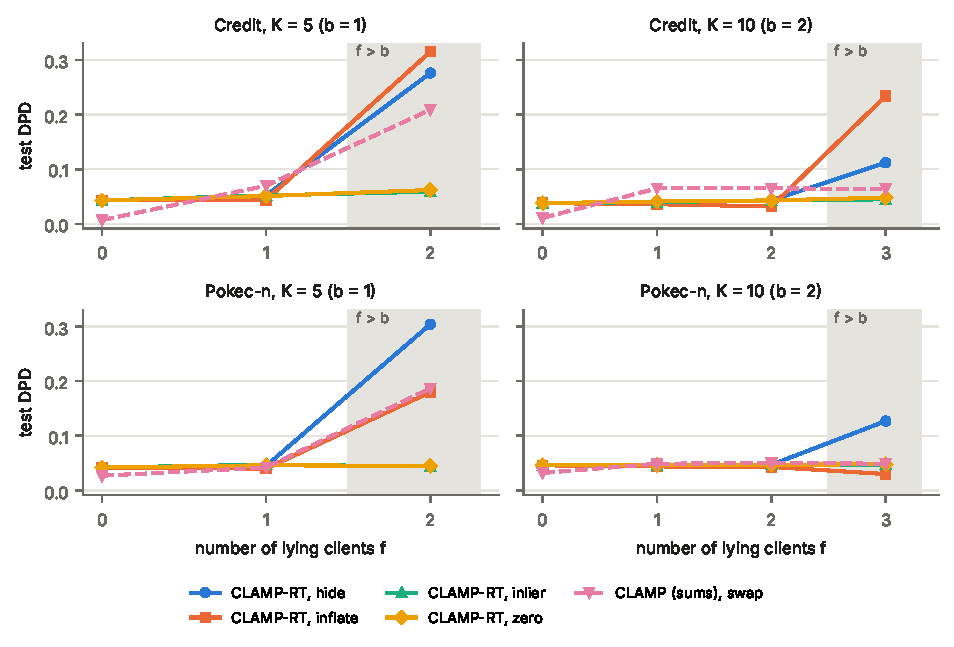
\includegraphics[width=\linewidth]{figures/fig_liars}
\caption{Test $\dpd$ against the number of lying clients $f$ (mean over 3 seeds). Shaded: $f>b$, beyond the breakdown point of the trimmed channel. Dashed: \clamp{} (sums channel, $P=1$) under the swap attack.}\label{fig:liars}
\end{figure}

\paragraph{Up to the breakdown point, the attacks do not move the outcome away from the honest level}
Table~\ref{tab:e4} and Figure~\ref{fig:liars} report the four gap attacks. For every dataset, $K$, attack and $f\le b$, the mean test gap stays within 0.009 of the honest run with the same seeds, which is less than its seed-to-seed standard deviation; the largest change is on Credit with $K=5$ and one hiding client (0.043 to 0.052). AUC changes by less than 0.01 (Table~S1). In all \nTthreeRounds{} attacked release rounds with $f\le b$ the pre-noise trimmed mean lay inside the interval of Theorem~\ref{thm:falsify}, as it must; this checks the implementation, not the theorem.

This result must be read together with the context columns of Table~\ref{tab:e4}. What the attacks fail to do is move the outcome away from the honest run; whether that honest run is itself well controlled is a separate question. On Credit it is: at $K=5$ the honest gap is 0.043 against 0.071 for ClipMean on the same seeds, the final multiplier is 0.14 and 53\% of the releases have $\Dhat>0$. On the Pokec graphs it is not: the honest gap is 0.041--0.046, the same as ClipMean where it was run (0.044 at $K=5$, 0.045 for Pokec-z at $K=10$), and the final multiplier is about 0.01. There the controller barely acts in the honest run, so an attack that leaves the gap unchanged shows only that the liars could not \emph{create} a problem, not that \rt{} would keep a large gap under control against them. On Bail the budget does not bind and the controller is inactive. Section~\ref{sec:adaptive} adds an adaptive attacker, repeats the study with per-round releases, where the controller is more active, and combines gap and update attacks.

\paragraph{Beyond the breakdown point, the hiding and inflating attacks succeed}
With $f=b+1$ one false value survives the trimming. The \emph{hide} attack, which reports a gap of full size with the opposite sign, then flips the sign of the estimate, and the controller pushes the model the wrong way: the gap rises to 0.276--0.304 with $K=5$ and to 0.112--0.127 with $K=10$ on Credit and the Pokec graphs, above the unconstrained level. The \emph{inflate} attack forces over-correction; on Credit it raises the gap to 0.315 ($K=5$) and 0.234 ($K=10$) and costs 0.09--0.14 AUC, on the Pokec graphs it raises the gap with $K=5$ (0.088 on Pokec-z, 0.180 on Pokec-n), whereas with $K=10$ it lowers the gap below the honest level (0.015 and 0.030) at a cost of about 0.01 AUC. In all runs beyond the breakdown point where the hide or inflate attack succeeded, the multiplier grew well beyond its honest level (final values 0.18--2.04, against at most 0.14 in the honest runs), and in 35 of the 96 runs beyond the breakdown point no release after the warm-up was feasible, so the last model was returned. The \emph{inlier} and \emph{zero} attacks, whose claims stay close to the honest values, have no clear effect even beyond the breakdown point (at most 0.062 against 0.043 on Credit). On Bail, where the budget does not bind, no attack has an effect.

\paragraph{Comparison with the sums channel}
Table~\ref{tab:oldnew} compares the two channels. With the sums channel a single liar out of ten raised the gap from \oldCreditKtenHon{} to \oldCreditKtenOne{} on Credit, from \oldPokeczKtenHon{} to \oldPokeczKtenOne{} on Pokec-z and from \oldPokecnKtenHon{} to \oldPokecnKtenOne{} on Pokec-n, i.e.\ to roughly the level of training without control, and additional liars did not change this. With the trimmed channel, one or two liars out of ten leave the gap at the honest level. The comparison has to be read with Table~\ref{tab:e1} in mind: because the honest level of \rt{} is itself higher, the attacked gap of \rt{} is lower than the attacked gap of \clamp{} only on Credit (0.041 against 0.065 for $f=1$, $K=10$); on the Pokec graphs the two are equal (0.046 against 0.045 and 0.049). What \rt{} gains is predictability: up to $b$ liars and against these fixed attacks, its fairness under attack was its fairness without attack, whatever that level was. With $K=5$ and two liars both channels fail.

\subsection{Adaptive, per-round and combined attacks}\label{sec:adaptive}

\begin{table}[tbp]
\centering
\footnotesize
\setlength{\tabcolsep}{3pt}
\caption{Adaptive gap attack (\emph{opt}: all liars report the common value that minimises the signed trimmed mean, Section~\ref{sec:setup}) at $P=10$: test DPD, mean$\pm$sd over 3 seeds. Honest: same seeds without liars (Table~\ref{tab:e4}). $\ast$: $f>b$. AUC in Table~S6.}
\label{tab:e7}
\begin{adjustbox}{max width=\textwidth}
\begin{tabular}{llcccc}
\toprule
Dataset & $K$ & Honest & $f=1$ & $f=2$ & $f=3$ \\
\midrule
Bail & 5 & 0.023$\pm$0.004 & 0.023$\pm$0.004 & 0.028$\pm$0.014$^\ast$ & -- \\
 & 10 & 0.008$\pm$0.002 & 0.009$\pm$0.002 & 0.009$\pm$0.002 & 0.006$\pm$0.007$^\ast$ \\
Credit & 5 & 0.043$\pm$0.019 & 0.052$\pm$0.014 & 0.275$\pm$0.028$^\ast$ & -- \\
 & 10 & 0.038$\pm$0.008 & 0.041$\pm$0.007 & 0.043$\pm$0.005 & 0.112$\pm$0.030$^\ast$ \\
Pokec-z & 5 & 0.041$\pm$0.004 & 0.042$\pm$0.006 & 0.279$\pm$0.029$^\ast$ & -- \\
 & 10 & 0.046$\pm$0.008 & 0.046$\pm$0.008 & 0.046$\pm$0.008 & 0.116$\pm$0.013$^\ast$ \\
Pokec-n & 5 & 0.042$\pm$0.012 & 0.045$\pm$0.011 & 0.304$\pm$0.031$^\ast$ & -- \\
 & 10 & 0.046$\pm$0.001 & 0.046$\pm$0.002 & 0.047$\pm$0.003 & 0.126$\pm$0.006$^\ast$ \\
\bottomrule
\end{tabular}
\end{adjustbox}
\end{table}

\begin{table}[tbp]
\centering
\scriptsize
\setlength{\tabcolsep}{3pt}
\caption{Gap attacks with per-round releases ($P=1$, $R=100$, $K=10$, $b=2$, $\varepsilon=8$): test DPD, mean over 3 seeds. Left block: honest runs at $P=1$ and, for comparison, at $P=10$ (Table~\ref{tab:e4}) and ClipMean on the same seeds where it was run; $\lambda^T$ and $\Dhat>0$ as in Table~\ref{tab:e4}. $f\le b$: largest mean DPD over the four attacks. $f=3>b$: each attack. Full table with sd and AUC: Table~S7.}
\label{tab:e8}
\begin{adjustbox}{max width=\textwidth}
\begin{tabular}{lccccc|cc|cccc}
\toprule
 & \multicolumn{5}{c|}{Honest} & \multicolumn{2}{c|}{worst, $f\le b$} & \multicolumn{4}{c}{$f=3$ (beyond breakdown)} \\
Dataset & $P=1$ & $\lambda^T$ & $\Dhat>0$ & $P=10$ & ClipMean & $f=1$ & $f=2$ & hide & inflate & inlier & opt \\
\midrule
Credit & 0.053 & 1.68 & 0.34 & 0.038 & -- & 0.059 & 0.059 & 0.096 & 0.066 & 0.053 & 0.095 \\
Pokec-z & 0.035 & 0.30 & 0.37 & 0.046 & 0.045 & 0.039 & 0.041 & 0.161 & 0.035 & 0.042 & 0.161 \\
Pokec-n & 0.037 & 0.30 & 0.36 & 0.046 & -- & 0.041 & 0.043 & 0.164 & 0.010 & 0.046 & 0.164 \\
\bottomrule
\end{tabular}
\end{adjustbox}
\end{table}


\paragraph{Adaptive attack}
The \emph{opt} attack lets all liars report the common value that minimises the signed noise-free trimmed mean, given all honest gaps and the public $b$; it is the myopically optimal single hiding claim. Table~\ref{tab:e7} reports it at $P=10$. For $f\le b$ it leaves the gap at the honest level, as the fixed attacks did: on Credit with $K=10$ it gives 0.041 and 0.043 for $f=1,2$ against 0.038 honest, on Pokec-z 0.046 against 0.046, and the largest change over all settings is again Credit with $K=5$ and $f=1$ (0.052 against 0.043). Beyond the breakdown point it does as much damage as the hiding attack: 0.275, 0.279 and 0.304 on Credit, Pokec-z and Pokec-n with $K=5$, $f=2$, and 0.112--0.126 with $K=10$, $f=3$. For $f\le b$ the optimal claim is an honest-range value, so by Theorem~\ref{thm:falsify} it can only shift the estimate within the interval; for $f>b$ it coincides in effect with the extreme claim of the hiding attack. The attack is a concrete strong attacker, not a proof of the worst case over all adaptive strategies: it uses one common value per release, it is myopic across releases, and it does not combine falsified gaps with poisoned updates.

\paragraph{Per-round releases}
With $P=10$ the multiplier on the Pokec graphs stayed near zero, so the attack study there could not show whether a working controller survives liars. Table~\ref{tab:e8} repeats it with $P=1$ ($R=100$ releases, hence a larger $\sigma_d$ of 0.049 on the Pokec graphs and 0.112 on Credit at $K=10$). The controller is now active: the final multiplier of the honest runs is \eEightPokeczLam{} on Pokec-z and \eEightPokecnLam{} on Pokec-n, against \eEightPtenPokeczLam{} and \eEightPtenPokecnLam{} at $P=10$, and \eEightCreditLam{} on Credit. On the Pokec graphs this lowers the honest gap from 0.046 to 0.035 and 0.037; on Pokec-z this is below ClipMean on the same seeds (0.045), so control has some effect, but the gap stays above the budget. On Credit the honest gap rises from 0.038 to 0.053: the larger noise of 100 releases drives the multiplier without bringing the gap down. Per-round releases therefore improve the honest level on the Pokec graphs and worsen it on Credit, consistent with the $K=5$ sweep of Table~\ref{tab:e5}.

Under attack with $f\le b$, the outcome again stays at the honest level: the largest mean gap over the hide, inflate, inlier and opt attacks is within 0.006 of the honest run on all three graphs. With an active controller this is a more meaningful result than at $P=10$: on the Pokec graphs the liars did not undo the reduction from 0.046 to 0.035--0.037 that the controller achieved. It remains a small reduction, and on Credit the controlled level is worse than at $P=10$. Beyond the breakdown point ($f=3$) the hiding and adaptive attacks raise the gap to 0.095--0.096 on Credit and 0.161--0.164 on the Pokec graphs, above ClipMean. The inflating attack at $f=3$ does not raise the gap (0.066 on Credit, 0.035 on Pokec-z, 0.010 on Pokec-n), but on Credit it drives the multiplier to 6.85 on average and lowers AUC from 0.753 to 0.724 $\pm$ 0.055. No ClipMean reference exists for Credit and Pokec-n at $K=10$.

\begin{table}[tbp]
\centering
\footnotesize
\setlength{\tabcolsep}{4pt}
\caption{Combined attack ($K=10$, $b=2$, $P=10$): the same $f$ clients poison their updates and report the adaptive \emph{opt} gap. Test DPD, mean over 3 seeds, as update-only $\to$ combined. Update-only references: Table~S2 (Bail, Pokec-z) and dedicated runs (Credit). $f=3>b$. Full table with sd and AUC: Table~S8.}
\label{tab:e9}
\begin{adjustbox}{max width=\textwidth}
\begin{tabular}{llccc}
\toprule
Dataset & Update attack & $f=1$ & $f=2$ & $f=3$ \\
\midrule
Bail & Fair.\ poison & 0.010 $\to$ 0.010 & 0.009 $\to$ 0.010 & 0.015 $\to$ 0.021 \\
 & Sign flip & 0.009 $\to$ 0.009 & 0.009 $\to$ 0.009 & 0.009 $\to$ 0.002 \\
 & ALIE & 0.010 $\to$ 0.010 & 0.007 $\to$ 0.007 & 0.006 $\to$ 0.005 \\
\midrule
Credit & Fair.\ poison & 0.040 $\to$ 0.044 & 0.045 $\to$ 0.051 & 0.051 $\to$ 0.138 \\
 & Sign flip & 0.037 $\to$ 0.041 & 0.036 $\to$ 0.046 & 0.038 $\to$ 0.112 \\
 & ALIE & 0.037 $\to$ 0.040 & 0.037 $\to$ 0.042 & 0.041 $\to$ 0.112 \\
\midrule
Pokec-z & Fair.\ poison & 0.059 $\to$ 0.062 & 0.118 $\to$ 0.122 & 0.151 $\to$ 0.212 \\
 & Sign flip & 0.043 $\to$ 0.042 & 0.032 $\to$ 0.032 & 0.025 $\to$ 0.062 \\
 & ALIE & 0.045 $\to$ 0.046 & 0.042 $\to$ 0.042 & 0.036 $\to$ 0.106 \\
\bottomrule
\end{tabular}
\end{adjustbox}
\end{table}


\paragraph{Combined update and gap attacks}
Table~\ref{tab:e9} lets the same $f$ clients poison their updates (fairness poisoning, sign flipping or ALIE) and report the adaptive \emph{opt} gap ($K=10$, $P=10$). For $f\le b=2$ the combined attack is close to the update attack alone: the largest increase is 0.010 (Credit, sign flipping, $f=2$: 0.036 to 0.046), on Pokec-z fairness poisoning gives 0.118 alone and 0.122 combined, and on Bail every change is within seed noise. This does not mean the protocol resists the update attack: fairness poisoning on Pokec-z already raises the gap to 0.118 without any false gap, as in Section~\ref{sec:byz}; the gap channel adds little on top. For $f=3>b$ the combination breaks the gap channel as the gap attack alone did: on Credit the gap rises from 0.041, 0.038 and 0.051 (ALIE, sign flipping, fairness poisoning alone) to 0.112, 0.112 and 0.138, and on Pokec-z from 0.036, 0.025 and 0.151 to 0.106, 0.062 and 0.212. On Bail, where the budget does not bind, $f=3$ changes little (fairness poisoning 0.015 to 0.021). The hiding and adaptive gap claims give the same results under fairness poisoning (Table~S8). The breakdown at $f>b$ is what Theorem~\ref{thm:falsify}, whose condition is $f\le b$, leaves open; the experiment shows that it is reached in practice, not that the theorem is tight.

\subsection{Update attacks and fairness poisoning}\label{sec:byz}

\begin{table}[tbp]
\centering
\scriptsize
\setlength{\tabcolsep}{3pt}
\caption{Fairness poisoning through updates ($K=10$): test DPD (AUC in parentheses), mean over 3 seeds. CLAMP (sums channel) uses $P=1$; $^\dagger$ needs individual updates and cannot run under secure aggregation. CLAMP-RT uses $P=10$.}
\label{tab:e3}
\begin{adjustbox}{max width=\textwidth}
\begin{tabular}{lcccccccc}
\toprule
Dataset & $f$ & FedAvg & Median$^\dagger$ & TrMean$^\dagger$ & Krum$^\dagger$ & ClipMean & CLAMP & CLAMP-RT \\
\midrule
Pokec-z & 0 & 0.035 (0.75) & 0.033 (0.75) & 0.035 (0.74) & 0.033 (0.74) & 0.045 (0.76) & 0.028 (0.76) & 0.046 (0.77) \\
 & 1 & 0.062 (0.75) & 0.046 (0.74) & 0.047 (0.73) & 0.035 (0.74) & 0.065 (0.76) & 0.025 (0.76) & 0.059 (0.77) \\
 & 2 & 0.124 (0.71) & 0.108 (0.72) & 0.146 (0.70) & 0.034 (0.72) & 0.137 (0.75) & 0.037 (0.72) & 0.118 (0.75) \\
 & 3 & 0.137 (0.70) & 0.148 (0.72) & 0.186 (0.69) & 0.035 (0.73) & 0.172 (0.74) & 0.049 (0.71) & 0.151 (0.74) \\
 & 4 & 0.137 (0.69) & 0.111 (0.72) & 0.201 (0.71) & 0.086 (0.71) & 0.125 (0.73) & 0.047 (0.71) & 0.106 (0.73) \\
\midrule
Bail & 0 & 0.011 (0.76) & 0.007 (0.73) & 0.013 (0.75) & 0.003 (0.72) & 0.009 (0.75) & 0.011 (0.75) & 0.009 (0.74) \\
 & 1 & 0.008 (0.75) & 0.008 (0.72) & 0.014 (0.74) & 0.005 (0.72) & 0.011 (0.74) & 0.012 (0.74) & 0.010 (0.74) \\
 & 2 & 0.014 (0.72) & 0.009 (0.72) & 0.010 (0.73) & 0.009 (0.71) & 0.010 (0.72) & 0.011 (0.72) & 0.009 (0.72) \\
 & 3 & 0.018 (0.71) & 0.010 (0.72) & 0.012 (0.73) & 0.005 (0.71) & 0.016 (0.72) & 0.009 (0.72) & 0.015 (0.71) \\
 & 4 & 0.021 (0.70) & 0.013 (0.71) & 0.014 (0.72) & 0.009 (0.71) & 0.023 (0.71) & 0.014 (0.72) & 0.023 (0.71) \\
\bottomrule
\end{tabular}
\end{adjustbox}
\end{table}


The trimmed channel does not change the update channel, and the results confirm it. Under the four update attacks that target utility, \rt{} behaves like the clipped mean (Table~S2): scaling has no effect because scaled updates are clipped; sign flipping lowers AUC gradually from 0.743 to 0.661 on Bail and from 0.768 to 0.710 on Pokec-z as $f$ grows from 0 to 4; ALIE and IPM cost at most 0.033 AUC.

Fairness poisoning is different (Table~\ref{tab:e3}). On Pokec-z it raises the gap of \rt{} to 0.118, 0.151 and 0.106 for $f=2,3,4$, close to ClipMean (0.137, 0.172, 0.125) and FedAvg (0.124--0.137). \clamp{} with per-round releases held the same attack at 0.037--0.049. In this respect \rt{} is a regression. The poisoning clients report their true gaps, so the gap channel does see the growing gap, but the multiplier of \rt{} reached at most 0.39 at the end of these runs, whereas that of \clamp{} reached 0.56--4.04 in eight of its nine runs with $f\ge2$. We attribute the difference mainly to the release period ($P=10$ gives the controller ten updates instead of a hundred), but we did not run \rt{} with $P=1$ under this attack, so this explanation is untested. Among the rules that need individual updates, only Krum held the gap (0.034--0.035 up to $f=3$). On Bail the attack raises the gap of every method by at most 0.014.

\subsection{Cost of the secure computation}\label{sec:mpc}

\begin{table}[tbp]
\centering
\footnotesize
\setlength{\tabcolsep}{4pt}
\caption{Measured cost of one release round of the server-side protocol in semi-honest two-party computation (CrypTen, two processes on one machine, local network; median of 3 repetitions). Bytes are those sent by one server as reported by CrypTen; rounds are communication rounds. Update channel: norm checks and masked sum of $K$ updates of dimension $d$. Gap channel: range checks, sort, trimmed mean and noise addition. Err: largest absolute fixed-point error of the trimmed mean (noise switched off), and of the update sum in the update block. The gap channel uses the validity bits of the update channel (a rejected update also removes the client's gap), so the full release round is the sum of the two blocks. Client-to-server input sharing and Beaver-triple generation are not included.}
\label{tab:mpc}
\begin{adjustbox}{max width=\textwidth}
\begin{tabular}{rrr rrrc rrrc rr}
\toprule
 & & & \multicolumn{4}{c}{Update channel} & \multicolumn{4}{c}{Gap channel} & \multicolumn{2}{c}{Full round} \\
$K$ & $b$ & $d$ & MB & rounds & s & Err & KB & rounds & s & Err & MB & s \\
\midrule
5 & 1 & $10^{4}$ & 2.56 & 12 & 0.79 & 4.5$\times10^{-7}$ & 9.3 & 64 & 0.33 & 5.9$\times10^{-6}$ & 2.57 & 1.12 \\
5 & 1 & $10^{5}$ & 25.60 & 12 & 1.44 & 3.2$\times10^{-3}$ & 9.3 & 64 & 0.30 & 1.0$\times10^{-5}$ & 25.61 & 1.74 \\
5 & 1 & $10^{6}$ & 256.00 & 12 & 3.12 & 1.0$\times10^{-3}$ & 9.3 & 64 & 0.33 & 1.5$\times10^{-5}$ & 256.01 & 3.44 \\
10 & 2 & $10^{4}$ & 4.96 & 12 & 0.88 & 9.1$\times10^{-7}$ & 30.2 & 109 & 0.54 & 1.0$\times10^{-5}$ & 4.99 & 1.42 \\
10 & 2 & $10^{5}$ & 49.60 & 12 & 1.33 & 3.2$\times10^{-3}$ & 30.2 & 109 & 0.51 & 1.1$\times10^{-5}$ & 49.63 & 1.84 \\
10 & 2 & $10^{6}$ & 496.00 & 12 & 4.51 & 1.0$\times10^{-3}$ & 30.2 & 109 & 0.42 & 6.4$\times10^{-6}$ & 496.03 & 4.94 \\
20 & 4 & $10^{4}$ & 9.77 & 12 & 0.73 & 1.6$\times10^{-6}$ & 106.7 & 199 & 0.92 & 9.7$\times10^{-6}$ & 9.88 & 1.65 \\
20 & 4 & $10^{5}$ & 97.61 & 12 & 1.47 & 5.4$\times10^{-7}$ & 106.7 & 199 & 1.12 & 1.2$\times10^{-5}$ & 97.72 & 2.59 \\
20 & 4 & $10^{6}$ & 976.01 & 12 & 9.55 & 1.0$\times10^{-3}$ & 106.7 & 199 & 0.95 & 1.5$\times10^{-5}$ & 976.12 & 10.50 \\
\bottomrule
\end{tabular}
\end{adjustbox}
\end{table}


We implemented the server step (validity checks, masked update sum, sort, trimming and noise) in CrypTen~\citep{knott2021crypten}: semi-honest two-party computation over $\mathbb{Z}_{2^{64}}$ with 16 fractional bits, Beaver triples from a trusted dealer, two processes on one machine, and an odd-even transposition sorting network ($K$ passes). Table~\ref{tab:mpc} reports one release round.

The gap channel itself does not depend on the model size. It takes 64, 109 and 199 communication rounds and 9.3, 30.2 and 106.7\,KB for $K=5$, 10 and 20 clients, and 0.30--1.12\,s on the local machine. It is not a stand-alone cost, however: a client's gap is used only if its update passes the norm check, so every release round also runs the update channel, which takes 12 rounds for any size and whose traffic grows linearly with $K\cdot d$. A full release round therefore costs \mpcTenMB\,MB and \mpcTenS\,s for $K=10$, $d=10^4$, and \mpcFullMB\,MB and \mpcFullS\,s for $K=20$, $d=10^6$, almost all of it in the update channel. The GAT backbones of our experiments have about $5\times10^3$ (Credit, Bail) to $4\times10^4$ (Facebook) parameters, computed from the layer shapes ($64\cdot\text{features}+4{,}545$ for two GAT layers with four heads of 16 units and a linear output), so $d=10^4$ is the representative row. Over a wide-area network the round count of the gap channel matters; at 50\,ms round-trip time, 199 rounds would add about 10\,s per release, a figure we computed and did not measure. The largest fixed-point error of the trimmed mean was $1.5\times10^{-5}$, about \mpcErrRatio{} times smaller than the smallest $\sigma_d$ in our runs (0.0128); the largest error of the update sum was $\mpcSumErrMax\times10^{-3}$ (for $d\ge10^5$), small against the norm bound $C=1$ but not negligible in every coordinate.

The measurement has clear limits. It is semi-honest, so a server that deviates from the protocol is not covered; ELSA-style malicious security~\citep{rathee2023elsa} would cost more. The trusted dealer and the clients' input sharing are not included. The noise was switched off in the error measurement, and the noise of the protocol is a continuous Gaussian sampled in floating point and then shared, not a discrete mechanism over the ring. A sorting network with lower depth than odd-even transposition would reduce the round count for larger $K$; we did not implement one. Finally, the training experiments did not run inside CrypTen; they execute the same arithmetic in plaintext.

\subsection{Privacy}\label{sec:privacy}

\begin{table}[tbp]
\centering
\footnotesize
\caption{Balanced accuracy of the optimal test that distinguishes two attribute-neighbouring datasets from the released gap (closed form, worst case $|\Delta|=\Delta_{\mathrm{TM}}$; $R=10$ releases, $\delta=10^{-5}$). $z=\sigma_d/\Delta_{\mathrm{TM}}$ from the RDP calibration. Both servers honest: one release with variance $2\sigma_d^2$. One server colluding: it removes its own noise. All releases: the colluding server combines all $R$ releases of a target whose contribution is unchanged. Bound: $(e^{\varepsilon}+\delta)/(1+e^{\varepsilon})$.}
\label{tab:attack}
\begin{adjustbox}{max width=\textwidth}
\begin{tabular}{cccccc}
\toprule
$\varepsilon$ & $z$ & Both honest, one release & One server, one release & One server, all $R$ & Bound \\
\midrule
1 & 12.79 & 0.511 & 0.516 & 0.549 & 0.7311 \\
2 & 6.80 & 0.521 & 0.529 & 0.592 & 0.8808 \\
4 & 3.66 & 0.538 & 0.554 & 0.667 & 0.9820 \\
8 & 2.02 & 0.570 & 0.598 & 0.783 & 0.9997 \\
\bottomrule
\end{tabular}
\end{adjustbox}
\end{table}

\begin{table}[tbp]
\centering
\scriptsize
\setlength{\tabcolsep}{3pt}
\caption{Privacy budget $\varepsilon$ of the gap channel and release period $P$ ($K=5$, 3 seeds): test DPD, mean$\pm$sd. Row $\infty$: no noise on the gap ($\sigma_d=0$, where the bias correction is the identity); these runs were made with $P\in\{1,10\}$ only. All other experiments use $\varepsilon=8$ and $P=10$.}
\label{tab:e5}
\begin{adjustbox}{max width=\textwidth}
\begin{tabular}{cccccccccc}
\toprule
 & \multicolumn{3}{c}{Credit} & \multicolumn{3}{c}{Pokec-z} & \multicolumn{3}{c}{Pokec-n} \\
$\varepsilon$ & $P=1$ & $P=5$ & $P=10$ & $P=1$ & $P=5$ & $P=10$ & $P=1$ & $P=5$ & $P=10$ \\
\midrule
1 & 0.057$\pm$0.022 & 0.057$\pm$0.007 & 0.063$\pm$0.005 & 0.051$\pm$0.027 & 0.056$\pm$0.012 & 0.046$\pm$0.007 & 0.055$\pm$0.039 & 0.055$\pm$0.026 & 0.048$\pm$0.009 \\
2 & 0.056$\pm$0.023 & 0.060$\pm$0.004 & 0.066$\pm$0.006 & 0.046$\pm$0.023 & 0.048$\pm$0.005 & 0.045$\pm$0.006 & 0.049$\pm$0.024 & 0.051$\pm$0.017 & 0.044$\pm$0.007 \\
4 & 0.061$\pm$0.019 & 0.063$\pm$0.003 & 0.049$\pm$0.027 & 0.030$\pm$0.004 & 0.045$\pm$0.002 & 0.039$\pm$0.006 & 0.032$\pm$0.005 & 0.043$\pm$0.004 & 0.043$\pm$0.012 \\
8 & 0.090$\pm$0.056 & 0.062$\pm$0.003 & 0.044$\pm$0.019 & 0.028$\pm$0.002 & 0.038$\pm$0.006 & 0.041$\pm$0.003 & 0.029$\pm$0.003 & 0.041$\pm$0.011 & 0.043$\pm$0.014 \\
\midrule
$\infty$ & 0.035$\pm$0.010 & -- & 0.048$\pm$0.008 & 0.017$\pm$0.007 & -- & 0.031$\pm$0.004 & 0.019$\pm$0.007 & -- & 0.029$\pm$0.006 \\
\bottomrule
\end{tabular}
\end{adjustbox}
\end{table}


\begin{figure}[tbp]
\centering
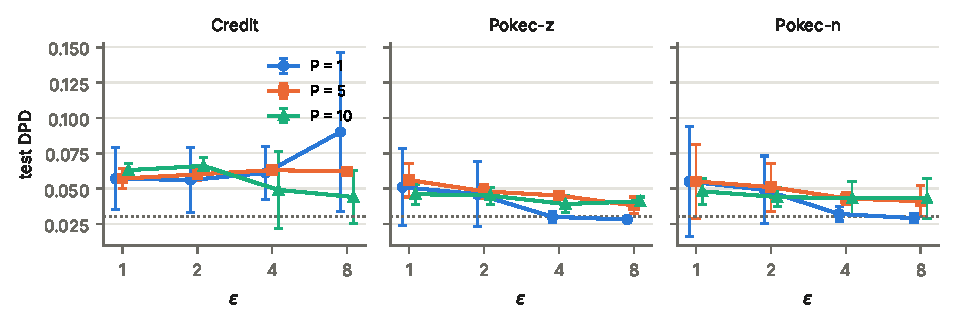
\includegraphics[width=\linewidth]{figures/fig_privacy}
\caption{Test $\dpd$ of \rt{} against the privacy budget of the gap channel for three release periods (mean $\pm$ sd over 3 seeds; dotted: budget $\tau=0.03$).}\label{fig:privacy}
\end{figure}

\paragraph{What the released gap reveals}
For a single release, the best test between two neighbouring datasets observes $\gt$ with mean $\TM$ or $\TM+\Delta$, $|\Delta|\le\DTM$, and noise $\mathcal{N}(0,2\sigma_d^2)$; its balanced accuracy is $\Phi(\Delta/(2\sqrt2\sigma_d))\le\Phi(1/(2\sqrt2 z))$, independent of the dataset because $\sigma_d=z\DTM$. Table~\ref{tab:attack} evaluates it. At $\varepsilon=8$ it is \accBothEight{} with both servers honest, \accOneEight{} if one server colludes and removes its own noise, and \accAllEight{} if the colluding server also combines all ten releases of a node whose contribution does not change, the worst case the accounting covers. The $(\varepsilon,\delta)$ bound, $(e^\varepsilon+\delta)/(1+e^\varepsilon)=\boundEight$, is uninformative at this level; the closed form is the more useful description. These values are for the worst case $|\Delta|=\DTM$; a node in a group much larger than $n_{0,k}$ changes the trimmed mean by less.

\paragraph{Privacy budget and release period}
Table~\ref{tab:e5} and Figure~\ref{fig:privacy} vary $\varepsilon$ and $P$. On Pokec-z and Pokec-n, per-round releases work best once $\varepsilon\ge4$ (0.028--0.032), matching \clamp{}, while $P=10$ stays at 0.039--0.043; at $\varepsilon\le2$ all periods give 0.044--0.056. Without noise ($\varepsilon=\infty$, last row) the Pokec graphs reach 0.017--0.019 at $P=1$ and about 0.03 at $P=10$. On Credit no noisy setting reaches the budget: the gap is 0.044--0.090, with the largest values and spread at $P=1$, $\varepsilon=8$ (0.090 $\pm$ 0.056), and at $\varepsilon\le4$ the results are noisy at every period. Even without noise the Credit gap is \nfCreditPone{} ($P=1$) and \nfCreditPten{} ($P=10$), so on Credit the noise is not the only cause of the shortfall (Section~\ref{sec:main}). AUC is \eFiveAucMin--\eFiveAucMax{} throughout the noisy runs (Table~S4). Our uniform choice $P=10$ is therefore not the best choice on the Pokec graphs. We nevertheless report all other experiments with $P=10$, because no single period was better on all three graphs; all attack studies and honest runs use $P=10$, and $K\in\{5,10\}$ only.

\paragraph{What the model reveals}
Theorem~\ref{thm:dp} does not cover the trained model. A separate probe study examined the final models of FedAvg, ClipMean and \clamp{} (last iterate) with a logistic-regression attribute probe on hidden representations: on German the probe reached AUC 0.86--0.87 for all three, against 0.85 for the raw features and 0.91 for an untrained GAT, and on Bail 0.54 against 0.61 for the raw features. We did not repeat the probe for \rt{}. Its model is trained by the same loop with a different multiplier, and we expect, but have not verified, similar values. Demographic-parity control does not remove the attribute from the representation, and neither protocol claims that it does.

\subsection{Ablations}\label{sec:ablation}

\begin{table}[tbp]
\centering
\footnotesize
\setlength{\tabcolsep}{3pt}
\caption{Ablations of the trimmed channel ($K=5$, $\varepsilon=8$, $P=10$, 3 seeds, honest). These runs use the variant without bias correction. $\sigma_d$ is the per-server noise standard deviation (mean$\pm$sd over seeds).}
\label{tab:e6}
\begin{adjustbox}{max width=\textwidth}
\begin{tabular}{l ccc ccc}
\toprule
 & \multicolumn{3}{c}{Credit} & \multicolumn{3}{c}{Pokec-z} \\
Variant & AUC & DPD & $\sigma_d$ & AUC & DPD & $\sigma_d$ \\
\midrule
Default ($b=1$, $c=0.05$) & 0.755$\pm$0.012 & 0.026$\pm$0.017 & 0.063$\pm$0.014 & 0.754$\pm$0.032 & 0.041$\pm$0.001 & 0.028$\pm$0.002 \\
Last iterate (no output rule) & 0.750$\pm$0.014 & 0.031$\pm$0.023 & 0.063$\pm$0.014 & 0.748$\pm$0.027 & 0.036$\pm$0.001 & 0.028$\pm$0.002 \\
$b=0$ (plain mean, no robustness) & 0.762$\pm$0.007 & 0.027$\pm$0.008 & 0.038$\pm$0.008 & 0.752$\pm$0.027 & 0.039$\pm$0.002 & 0.017$\pm$0.001 \\
$b=2$ (median of $K=5$) & 0.683$\pm$0.041 & 0.168$\pm$0.048 & 0.188$\pm$0.042 & 0.752$\pm$0.038 & 0.039$\pm$0.021 & 0.084$\pm$0.005 \\
$c=0.2$ & 0.657$\pm$0.004 & 0.236$\pm$0.008 & 0.016$\pm$0.004 & 0.753$\pm$0.026 & 0.033$\pm$0.004 & 0.007$\pm$0.000 \\
\bottomrule
\end{tabular}
\end{adjustbox}
\end{table}


Table~\ref{tab:e6} varies the trimming level, the floor fraction and the output rule on Credit and Pokec-z (variant without bias correction, three seeds). Trimming costs little in honest runs: the plain mean ($b=0$) has a smaller $\sigma_d$ (0.038 against 0.063 on Credit) and a gap within seed noise of the default (0.027 against 0.026). Two settings are clearly bad. With $b=2$ at $K=5$ the statistic is the median, its sensitivity triples ($\sigma_d=0.188$ on Credit), and the Credit gap rises to 0.168 with AUC 0.683. With $c=0.2$ the noise is smaller ($\sigma_d=0.016$), but the Credit gap is 0.236 with AUC 0.657. The likely reason is the floor: the protected group is 9\% of Credit's nodes, so with $c=0.2$ it is smaller than $n_{0,k}$ on most clients, its rate is shrunk toward zero, and the estimated gap is biased in one direction; on Pokec-z, whose groups are larger than the floor, $c=0.2$ works (0.033). The floor fraction must therefore stay below the smallest group share, which is a constraint the federation has to set from public knowledge. Returning the last iterate instead of the stored model changes the Credit gap by less than the seed noise (0.031 $\pm$ 0.023 against 0.026 $\pm$ 0.017), but on Pokec-z the last iterate is better than the stored model (0.036 $\pm$ 0.001 against 0.041 $\pm$ 0.001), a difference larger than the seed spread: with the looser feasibility test of the corrected variant and few releases, the output rule does not always pick a better model than the last one.

\paragraph{Discarded variants}
Table~S5 in the supplementary material lists all development pilots (two seeds each, among seeds 0--2): the initial floor fraction $c=0.1$, exponential smoothing of the released gap (EMA, factor 0.3), a multiplier step scaled by the release period, a tighter controller target $\tau_c=0.02$, and the first runs of the bias correction. None of them was adopted. Some of them were not worse in these small pilots; for example the noisy Credit pilot with $c=0.1$ and $P=10$ gave 0.023 against 0.025 for $c=0.05$, with two seeds each. The adopted configuration is therefore a choice among similar pilots, not a tuned optimum, and the pilots share seeds with the reported runs.

\section{Discussion and limitations}\label{sec:discussion}

\paragraph{What the trimmed channel buys and what it costs}
The trimmed channel answers the main weakness of the sums channel: up to $b$ liars cannot move the noise-free fairness estimate outside the range of honest values (Theorem~\ref{thm:falsify}), and in our fixed attacks they did not move the test gap away from the honest level. With ten releases that level was close to training without control on the Pokec graphs. With per-round releases the multiplier was active and lowered the Pokec gaps from 0.046 to 0.035--0.037, and liars with $f\le b$, including the adaptive attacker, did not undo this. The reduction is small and the gap stays above the budget, so the evidence is for robustness of a weak controller, not of a strong one. The price is paid in the honest case. A trimmed mean of $K$ per-client gaps has sensitivity $2/(n_{0,\min}(K-2b))$, which is set by the smallest client's validation set, whereas the pooled gap of \clamp{} had a sensitivity set by pooled counts. At the same $\varepsilon$ the trimmed channel is noisier, and with ten releases it controlled the gap less tightly than \clamp{} on Credit and the Pokec graphs. A federation that expects no liars has no reason to prefer \rt{}; one that cannot rule out a minority of liars obtains bounded behaviour at a higher, but predictable, gap.

\paragraph{The proxy}
The controller acts on a trimmed mean of per-client gaps, not on the pooled gap. Under strongly non-IID partitions the two can differ, and a client whose local gap has the opposite sign to the pooled one pulls the estimate the wrong way even when honest. The noise-free runs indicate that this matters on Credit, where even noise-free per-round releases leave the gap at 0.035, against 0.007 for the pooled channel on the same seeds, whereas on the Pokec graphs the noise-free trimmed channel matches or beats the pooled one. We have not isolated the proxy effect (for example by evaluating the noise-free trimmed statistic and the pooled gap on the same trajectory), so this attribution is a likely explanation, not a measurement. A robust estimate of the pooled gap would need robust aggregation of per-client rate pairs, weighted by group sizes that are themselves sensitive; we leave this open.

\paragraph{Breakdown and the choice of $b$}
Robustness holds only for $f\le b$, and beyond it the hiding attack turns the controller against its purpose (Section~\ref{sec:statattack}). Larger $b$ raises the breakdown point but also the sensitivity: at $K=5$, $b=2$ already made the channel unusable on Credit. Small federations therefore cannot tolerate more than one liar with this design, and $b$ must be chosen from an assumption about $f$ that the protocol cannot verify.

\paragraph{Small graphs}
With 20--40 validation nodes on the smallest client, the floor $n_{0,\min}$ is 1 or 2 and the noise at $\varepsilon=8$ exceeds any gap. On German, NBA and Facebook the controller of \rt{} acts on noise, and the improvement of the bias-corrected variant over the uncorrected one there is mostly an effect of the output rule. Larger validation sets, a lower privacy level for the gap channel, or excluding clients with tiny validation sets from the floor would be needed; each has costs we have not evaluated.

\paragraph{Fairness poisoning through updates}
The trimmed channel does not touch the update channel. Under fairness poisoning on Pokec-z, \rt{} behaved like clipped aggregation without control, whereas \clamp{} with per-round releases held the gap. The slower controller is the likely cause, and the privacy sweep suggests that per-round releases would help on Pokec, but we have not tested this under attack. When the same clients also falsify their gaps, the outcome for $f\le b$ is about the same as the update attack alone, and for $f>b$ it is worse (Section~\ref{sec:adaptive}). Combining the robust gap channel with a faster controller, or with robust aggregation of updates in secure computation, is an open problem.

\paragraph{Secure computation and noise}
The training experiments simulate the two-party protocol in plaintext, and its cost was measured separately in a semi-honest setting with a trusted dealer. A deployment needs a maliciously secure protocol if the servers cannot be trusted to follow it, input validation of the shares, and a discrete noise mechanism over the ring, for which the sensitivity must include fixed-point rounding and the privacy accounting of Theorem~\ref{thm:dp} must be redone~\citep{canonne2020discrete,kairouz2021distributed}. We do not claim that our continuous-noise analysis transfers unchanged.

\paragraph{Scope of privacy}
Theorem~\ref{thm:dp} protects the attribute of each validation node with respect to the released gaps. It does not protect training-node attributes, which enter the update sum, and it does not make the model differentially private. The value $\varepsilon=8$ gives a weak worst-case bound; the closed-form attack accuracy of Table~\ref{tab:attack} (0.57--0.78 at $\varepsilon=8$, depending on collusion and on how many releases the attacker combines) is a more concrete description.

\paragraph{Guarantees that hold only for the noise-free statistic}
Theorem~\ref{thm:falsify} and its consequences concern $\TM(\tilde d)$ before noise. The controller sees the bias-corrected magnitude, which is zero whenever $|\gt|\le\sqrt2\sigma_d$ (0.065--0.100 on Credit, above the budget), so ``liars cannot hide a gap that all honest clients see'' does not imply ``the controller responds to it''. At $f=b$ the condition of consequence (ii) requires every honest client to see the gap.

\paragraph{Scope of the experiments}
The attack studies, the privacy sweep and the ablations use three seeds, so only large differences are meaningful there. The attack studies use $K\in\{5,10\}$, $P=10$, and for $K=10$ on three graphs also $P=1$; none uses more clients. The adaptive attack is myopic and uses one common claim per release; it is not a worst case over all adaptive strategies. The combined attack (poisoned updates and the adaptive gap claim from the same clients) was run only at $K=10$, $P=10$ on three graphs. The output-rule fallback rate matters for Theorem~\ref{thm:output}, which is conditional on no fallback; it was zero in the honest runs, 7 of 126 in the update-attack runs and 35 of 96 in the falsification runs beyond the breakdown point. On German the result is highly variable (0.172 $\pm$ 0.189 over ten seeds), so a mean comparison there says little. The attribute probe on the final model was not repeated for \rt{}; the values we cite are for \clamp{}, FedAvg and ClipMean. All statistics attacks are omniscient but use simple fixed strategies; the adaptive \emph{opt} attack did no more damage than the fixed hiding attack in our settings. A stronger adaptive adversary may exist, but for $f\le b$ it cannot place the noise-free estimate outside the interval of Theorem~\ref{thm:falsify}, although it can choose its position within that interval in every release. We evaluated one binary attribute and demographic parity only.

\section{Conclusion}\label{sec:conclusion}

\rt{} replaces the summed group statistics of the sums-based \clamp{} design by one secret-shared scalar per client, sorted, trimmed and privatised by two non-colluding servers. We proved that up to $b$ falsifying clients cannot move the released estimate outside the range of honest gaps, that the release is attribute-level differentially private with a sensitivity fixed by public validation-set sizes, and a high-probability bound on the released gap of the returned model. In experiments with four fixed attacks and an adaptive one, up to $b$ liars did not move the test gap away from its honest level, where one liar had disabled the sums-based \clamp{}. With ten releases that honest level was close to training without control on the Pokec graphs; with per-round releases the controller was active, lowered the gap modestly, and liars with $f\le b$ again did not change the outcome. Liars that also poisoned their updates added little to the update attack when $f\le b$ and broke the gap channel when $f>b$. A full release round cost 1.1--10.5\,s in a semi-honest two-party implementation, dominated by the norm checks on the updates.

The design has clear costs and limits. With noise on a single trimmed scalar and ten releases, the honest-case gap on Credit and the Pokec graphs was higher than with the sums-based \clamp{}; on graphs with a few hundred nodes the noise exceeds the signal; robustness ends at $f=b+1$, where a hiding attack turns the controller against its purpose; fairness poisoning through updates is not countered; and the training experiments simulate the secure computation with continuous noise. Making the robust channel as accurate as the pooled one, and pairing it with a robust update channel, remain open.


\section*{Data and code availability}
All eight datasets are public benchmarks (German, Bail, Credit, Pokec-z, Pokec-n, NBA, Facebook and AMiner-S). The code, the configuration files, the per-run results with per-round logs, and the scripts that generate every table and figure of this paper are available upon publication.

\bibliographystyle{elsarticle-num}
\bibliography{ref}

\end{document}
